\documentclass[12pt,a4paper]{article}
\usepackage[utf8]{inputenc}
\usepackage[french]{babel}
\usepackage[T1]{fontenc}
\usepackage{amsmath,amsfonts,amssymb}
\usepackage{graphicx}
\usepackage{enumitem}
\usepackage{array}
\usepackage{booktabs}
\usepackage{multirow}
\usepackage{geometry}
\usepackage{fancyhdr}
\usepackage{color,xcolor}
\usepackage{tikz}
\usepackage{pgfplots}
\usepackage{listings}
\usepackage{algorithm}
\usepackage{algorithmic}
\usepackage{subcaption}
\usepackage{float}
\usepackage{hyperref}
\usepackage{listings}
\usepackage{xcolor}

\lstset{
    language=Python,
    basicstyle=\ttfamily\footnotesize,
    keywordstyle=\color{blue},
    stringstyle=\color{red},
    commentstyle=\color{green!50!black},
    showstringspaces=false,
    frame=single,
    breaklines=true
}

\geometry{left=2.5cm,right=2.5cm,top=3cm,bottom=3cm}
\pagestyle{fancy}
\fancyhf{}
\fancyhead[L]{Analyse VGG-11 CIFAR-10}
\fancyhead[R]{\today}
\fancyfoot[C]{\thepage}

\definecolor{codeblue}{rgb}{0.25,0.5,0.75}
\definecolor{codegray}{rgb}{0.5,0.5,0.5}
\definecolor{vggcolor}{rgb}{0.8,0.2,0.2}
\usepackage{pgfplots}
\pgfplotsset{compat=1.18}
\lstdefinestyle{pythonstyle}{
    language=Python,
    basicstyle=\ttfamily\footnotesize,
    commentstyle=\color{codegray},
    keywordstyle=\color{codeblue},
    stringstyle=\color{red},
    numbers=left,
    numberstyle=\tiny\color{codegray},
    stepnumber=1,
    numbersep=5pt,
    backgroundcolor=\color{gray!10},
    showspaces=false,
    showstringspaces=false,
    showtabs=false,
    frame=single,
    rulecolor=\color{black},
    tabsize=2,
    captionpos=b,
    breaklines=true,
    breakatwhitespace=false,
    escapeinside={\%*}{*)}
}

\title{\textbf{Architecture VGG-11 Adaptée pour CIFAR-10} \\
\large{Analyse Technique et Évaluation des Choix de Conception}}

\author{Analyse Architecturale Approfondie}
\date{\today}

\begin{document}

\maketitle

\begin{abstract}
Cette étude présente une analyse détaillée d'une architecture VGG-11 modifiée et optimisée pour la classification d'images CIFAR-10. Le modèle proposé intègre des techniques modernes de régularisation tout en conservant la philosophie architecturale VGG. L'architecture comprend 8 couches convolutionnelles organisées en 4 blocs, suivies d'un classificateur dense à 3 couches, totalisant approximativement 9.8 millions de paramètres avec des optimisations spécifiques pour des images de faible résolution.
\end{abstract}

\tableofcontents
\newpage

\section{Introduction}

L'architecture VGG (Visual Geometry Group), introduite par Simonyan et Zisserman en 2014, a révolutionné le domaine de la vision par ordinateur en démontrant l'efficacité des réseaux profonds avec des filtres de petite taille. Cette étude analyse une adaptation moderne de VGG-11 spécifiquement conçue pour le dataset CIFAR-10, intégrant des techniques de régularisation contemporaines et des optimisations architecturales.
\section{Analyse du modèle existant}
\subsection{Description Architecturale Générale}

\subsubsection{Philosophie de Conception}

L'architecture proposée s'inspire du paradigme VGG classique tout en intégrant des améliorations modernes :

\begin{itemize}
    \item \textbf{Filtres uniformes} : Utilisation exclusive de noyaux $3 \times 3$
    \item \textbf{Profondeur contrôlée} : 8 couches convolutionnelles (vs 11 dans VGG-11 original)
    \item \textbf{Régularisation moderne} : BatchNormalization et SpatialDropout2D
    \item \textbf{Adaptation CIFAR-10} : Optimisation pour images $32 \times 32$ pixels
\end{itemize}

\subsubsection{Structure Hiérarchique}

Le modèle est organisé en une structure pyramidale à 4 niveaux :

\begin{enumerate}
    \item \textbf{Bloc 1} : Extraction des caractéristiques de bas niveau (32 filtres)
    \item \textbf{Bloc 2} : Consolidation des motifs élémentaires (32 filtres)
    \item \textbf{Bloc 3} : Capture des motifs intermédiaires (64 filtres)
    \item \textbf{Bloc 4} : Extraction des caractéristiques de haut niveau (128 filtres)
\end{enumerate}

\subsection{Analyse Détaillée par Blocs}

\subsubsection{Bloc Convolutionnel 1 : Extraction Primaire}

\begin{align}
\mathbf{X}_1 &= \text{Conv2D}(\mathbf{X}_0, \mathbf{W}_1) \quad \text{où } \mathbf{W}_1 \in \mathbb{R}^{32 \times 3 \times 3 \times 3} \\
\mathbf{X}_1^{act} &= \text{ReLU}(\mathbf{X}_1) \\
\mathbf{X}_1^{norm} &= \text{BatchNorm}(\mathbf{X}_1^{act})
\end{align}

\textbf{Caractéristiques techniques :}
\begin{itemize}
    \item Entrée : $(3, 32, 32)$ → Sortie : $(32, 32, 32)$
    \item Champ récepteur : $3 \times 3$
    \item Paramètres : $3 \times 3 \times 3 \times 32 + 32 = 896$
\end{itemize}

\subsubsection{Bloc Convolutionnel 2 : Consolidation avec Régularisation}

\begin{align}
\mathbf{X}_2 &= \text{Conv2D}(\mathbf{X}_1^{norm}, \mathbf{W}_2) \quad \text{où } \mathbf{W}_2 \in \mathbb{R}^{32 \times 32 \times 3 \times 3} \\
\mathbf{X}_2^{act} &= \text{ReLU}(\mathbf{X}_2) \\
\mathbf{X}_2^{drop} &= \text{SpatialDropout2D}(\mathbf{X}_2^{act}, p=0.25) \\
\mathbf{X}_2^{norm} &= \text{BatchNorm}(\mathbf{X}_2^{drop}) \\
\mathbf{X}_2^{pool} &= \text{MaxPool2D}(\mathbf{X}_2^{norm}, k=2, s=2)
\end{align}

\textbf{Innovation architecturale :} Introduction du SpatialDropout2D préservant les corrélations spatiales.

\textbf{Transformation dimensionnelle :} $(32, 32, 32)$ → $(32, 16, 16)$

\subsubsection{Blocs Convolutionnels 3-4 : Montée en Abstraction}

Les blocs 3 et 4 suivent un pattern similaire avec progression des canaux :

\begin{table}[H]
\centering
\caption{Progression des caractéristiques par bloc}
\begin{tabular}{cccc}
\toprule
\textbf{Bloc} & \textbf{Canaux d'entrée} & \textbf{Canaux de sortie} & \textbf{Dimension spatiale} \\
\midrule
1 & 3 & 32 & $32 \times 32$ \\
2 & 32 & 32 & $32 \times 32 \rightarrow 16 \times 16$ \\
3 & 32 & 64 & $16 \times 16$ \\
4 & 64 & 64 & $16 \times 16 \rightarrow 8 \times 8$ \\
5 & 64 & 128 & $8 \times 8 \rightarrow 4 \times 4$ \\
6 & 128 & 128 & $4 \times 4 \rightarrow 2 \times 2$ \\
\bottomrule
\end{tabular}
\end{table}

\subsubsection{Classificateur Dense}

La phase de classification suit une réduction pyramidale :

\begin{align}
\mathbf{f} &= \text{Flatten}(\mathbf{X}_6^{pool}) \in \mathbb{R}^{512} \quad (128 \times 2 \times 2) \\
\mathbf{h}_1 &= \text{ReLU}(\mathbf{W}_7 \mathbf{f} + \mathbf{b}_7) \in \mathbb{R}^{1024} \\
\mathbf{h}_1^{drop} &= \text{Dropout}(\mathbf{h}_1, p=0.3) \\
\mathbf{h}_2 &= \text{ReLU}(\mathbf{W}_8 \mathbf{h}_1^{drop} + \mathbf{b}_8) \in \mathbb{R}^{512} \\
\mathbf{h}_2^{drop} &= \text{Dropout}(\mathbf{h}_2, p=0.3) \\
\mathbf{y} &= \text{Softmax}(\mathbf{W}_9 \mathbf{h}_2^{drop} + \mathbf{b}_9) \in \mathbb{R}^{10}
\end{align}

\subsection{Analyse des Innovations Architecturales}

\subsubsection{BatchNormalization Stratégique}

L'intégration de la BatchNormalization après chaque activation présente plusieurs avantages :

\begin{itemize}
    \item \textbf{Stabilisation} : Réduction de la variance interne des activations
    \item \textbf{Accélération} : Convergence plus rapide durant l'entraînement
    \item \textbf{Régularisation} : Effet implicite de régularisation
    \item \textbf{Robustesse} : Moins de sensibilité à l'initialisation
\end{itemize}

\textbf{Formulation mathématique :}
$$\hat{x}_i = \frac{x_i - \mu_{\mathcal{B}}}{\sqrt{\sigma_{\mathcal{B}}^2 + \epsilon}} \cdot \gamma + \beta$$

\subsubsection{SpatialDropout2D : Innovation Spatiale}

Le SpatialDropout2D constitue une amélioration significative par rapport au dropout classique :

\begin{table}[H]
\centering
\caption{Comparaison Dropout classique vs SpatialDropout2D}
\begin{tabular}{lcc}
\toprule
\textbf{Caractéristique} & \textbf{Dropout Classique} & \textbf{SpatialDropout2D} \\
\midrule
Unité de suppression & Neurones individuels & Canaux complets \\
Préservation spatiale & Non & Oui \\
Corrélations locales & Perturbées & Maintenues \\
Efficacité convolutionnelle & Limitée & Optimale \\
\bottomrule
\end{tabular}
\end{table}

\subsubsection{Ordre des Opérations Optimisé}

L'architecture propose un ordre d'opérations innovant :

\textbf{Séquence proposée :} Conv2D → ReLU → [SpatialDropout2D] → BatchNorm → [MaxPool2D]

Cette séquence présente l'avantage de normaliser les activations après application du dropout, stabilisant ainsi la distribution des données d'entrée de la couche suivante.

\subsection{Analyse Quantitative des Paramètres}

\subsubsection{Distribution Paramétrique Détaillée}

\begin{table}[H]
\centering
\caption{Répartition complète des paramètres}
\begin{tabular}{lrrr}
\toprule
\textbf{Composant} & \textbf{Paramètres} & \textbf{Pourcentage} & \textbf{Calcul} \\
\midrule
\multicolumn{4}{c}{\textit{Couches Convolutionnelles}} \\
Conv2D (3→32) & 896 & 0.009\% & $3 \times 3 \times 3 \times 32 + 32$ \\
Conv2D (32→32) & 9,248 & 0.094\% & $3 \times 3 \times 32 \times 32 + 32$ \\
Conv2D (32→64) & 18,496 & 0.189\% & $3 \times 3 \times 32 \times 64 + 64$ \\
Conv2D (64→64) & 36,928 & 0.377\% & $3 \times 3 \times 64 \times 64 + 64$ \\
Conv2D (64→128) & 73,856 & 0.754\% & $3 \times 3 \times 64 \times 128 + 128$ \\
Conv2D (128→128) & 147,584 & 1.507\% & $3 \times 3 \times 128 \times 128 + 128$ \\
\midrule
\multicolumn{4}{c}{\textit{BatchNormalization}} \\
BN (32 canaux) × 2 & 128 & 0.001\% & $(32 + 32) \times 2$ \\
BN (64 canaux) × 2 & 256 & 0.003\% & $(64 + 64) \times 2$ \\
BN (128 canaux) × 2 & 512 & 0.005\% & $(128 + 128) \times 2$ \\
\midrule
\multicolumn{4}{c}{\textit{Couches Denses}} \\
Dense (512→1024) & 525,312 & 5.368\% & $512 \times 1024 + 1024$ \\
Dense (1024→512) & 524,800 & 5.363\% & $1024 \times 512 + 512$ \\
Dense (512→10) & 5,130 & 0.052\% & $512 \times 10 + 10$ \\
\midrule
\textbf{Total Estimé} & \textbf{env 1,343,146} & \textbf{100\%} & \\
\bottomrule
\end{tabular}
\end{table}

\subsubsection{Analyse de l'Efficacité Paramétrique}

\begin{figure}[H]
\centering
\begin{tikzpicture}
\begin{axis}[
    width=12cm, height=8cm,
    ybar,
    bar width=15pt,
    ylabel={Pourcentage des paramètres (\%)},
    symbolic x coords={Conv, BatchNorm, Dense},
    xtick=data,
    nodes near coords,
    nodes near coords align={vertical},
    ymin=0, ymax=12,
    title={Distribution des paramètres par type de couche}
]
\addplot coordinates {(Conv,2.93) (BatchNorm,0.009) (Dense,10.78)};
\end{axis}
\end{tikzpicture}
\caption{Répartition des paramètres dans l'architecture VGG-11 CIFAR-10}
\end{figure}

\textbf{Observations critiques :}
\begin{itemize}
    \item \textbf{78.3\%} des paramètres dans le classificateur dense
    \item Meilleur équilibre que l'architecture CNN précédemment analysée
    \item Les couches convolutionnelles représentent \textbf{21.7\%} des paramètres
\end{itemize}

\subsection{Comparaison avec l'Architecture VGG Originale}

\subsubsection{Adaptations pour CIFAR-10}

\begin{table}[H]
\centering
\caption{VGG-11 Original vs VGG-11 CIFAR-10 Adapté}
\begin{tabular}{lcc}
\toprule
\textbf{Aspect} & \textbf{VGG-11 Original} & \textbf{Version CIFAR-10} \\
\midrule
Résolution d'entrée & $224 \times 224$ & $32 \times 32$ \\
Nombre de couches conv & 8 & 8 \\
Filtres max & 512 & 128 \\
Taille classificateur & 25,088 → 4,096 → 4,096 → 1,000 & 512 → 1,024 → 512 → 10 \\
BatchNormalization & Non & Oui \\
SpatialDropout & Non & Oui \\
Paramètres totaux & 132M & 1.34M \\
\bottomrule
\end{tabular}
\end{table}

\subsubsection{Justifications des Modifications}

\subsubsection{Réduction de la Complexité des Filtres}

La limitation à 128 filtres maximum s'explique par :
\begin{itemize}
    \item \textbf{Résolution d'entrée réduite} : $32 \times 32$ vs $224 \times 224$
    \item \textbf{Complexité du dataset} : CIFAR-10 (10 classes) vs ImageNet (1000 classes)
    \item \textbf{Prévention du sur-apprentissage} : Capacité adaptée aux données disponibles
\end{itemize}

\subsubsection{Intégration de la Régularisation Moderne}

L'ajout de BatchNorm et SpatialDropout répond à plusieurs objectifs :
\begin{itemize}
    \item \textbf{Stabilité d'entraînement} : BatchNorm réduit la dépendance à l'initialisation
    \item \textbf{Généralisation} : SpatialDropout prévient le sur-apprentissage spatial
    \item \textbf{Performance} : Accélération de la convergence
\end{itemize}

\subsection{Analyse des Performances Attendues}

\subsubsection{Estimation Théorique}

Basé sur l'architecture et les techniques employées :

\begin{table}[H]
\centering
\caption{Prédictions de performance}
\begin{tabular}{ll}
\toprule
\textbf{Métrique} & \textbf{Estimation} \\
\midrule
Accuracy CIFAR-10 & 88-93\% \\
Époques de convergence & 50-80 \\
Temps d'entraînement & Modéré \\
Stabilité & Élevée (BatchNorm) \\
Généralisation & Bonne (régularisation multiple) \\
Robustesse & Élevée (architecture éprouvée) \\
\bottomrule
\end{tabular}
\end{table}

\subsubsection{Comparaison avec Architectures de Référence}

\begin{table}[H]
\centering
\caption{Benchmarking architectural}
\begin{tabular}{lccc}
\toprule
\textbf{Architecture} & \textbf{Paramètres} & \textbf{CIFAR-10 Acc.} & \textbf{Complexité} \\
\midrule
LeNet-5 & 60K &  70\% & Faible \\
AlexNet Adapté & 2M & 85\% & Moyenne \\
\textbf{VGG-11 CIFAR-10} & \textbf{1.34M} & \textbf{90\%} & \textbf{Moyenne} \\
ResNet-20 & 270K &  92\% & Moyenne \\
DenseNet-40 & 1M &  94\% & Élevée \\
\bottomrule
\end{tabular}
\end{table}

\subsection{Recommandations d'Optimisation}

\subsubsection{Améliorations Architecturales}

\paragraph{Connexions Résiduelles}

L'intégration de skip connections pourrait améliorer les performances :

\begin{lstlisting}[style=pythonstyle, caption=Bloc VGG avec connexions résiduelles]
def vgg_residual_block(x, filters):
    # Couche principale
    y = layers.Conv2D(filters, (3,3), padding='same')(x)
    y = layers.Activation('relu')(y)
    y = layers.BatchNormalization()(y)
    
    # Skip connection si dimensions compatibles
    if x.shape[-1] == filters:
        return layers.Add()([x, y])
    else:
        
        shortcut = layers.Conv2D(filters, (1,1), padding='same')(x)
        return layers.Add()([shortcut, y])
\end{lstlisting}

\subsubsection{Attention Spatiale}

L'ajout de mécanismes d'attention pourrait cibler les régions discriminantes :

$$\text{Attention}(\mathbf{F}) = \sigma(\text{Conv}_{1 \times 1}(\text{GAP}(\mathbf{F}) + \text{GMP}(\mathbf{F})))$$

\subsubsection{Optimisations d'Entraînement}

\begin{enumerate}
    \item \textbf{Learning Rate Scheduling} : Décroissance cosine ou step decay
    \item \textbf{Data Augmentation} : Rotation, translation, cutout
    \item \textbf{Label Smoothing} : Réduction du sur-apprentissage sur les labels
    \item \textbf{Mixed Precision} : Accélération avec maintien de la précision
\end{enumerate}

\subsection{Limitations et Défis}

\subsubsection{Limitations Architecturales}

\begin{itemize}
    \item \textbf{Absence de skip connections} : Limite la profondeur effective
    \item \textbf{Pooling agressif} : Perte d'information spatiale fine
    \item \textbf{Architecture séquentielle} : Pas de parallélisation des branches
\end{itemize}

\subsubsection{Défis Computationnels}

\begin{itemize}
    \item \textbf{Mémoire} : Stockage des cartes de caractéristiques volumineuses
    \item \textbf{BatchNorm} : Dépendance à la taille du batch
    \item \textbf{Régularisation} : Équilibrage dropout/BatchNorm
\end{itemize}

\subsection{Conclusion}

L'architecture VGG-11 adaptée pour CIFAR-10 présente une modernisation réussie du paradigme VGG classique. Les principales innovations incluent :

\begin{enumerate}
    \item \textbf{Intégration harmonieuse} de la BatchNormalization
    \item \textbf{Utilisation innovante} du SpatialDropout2D
    \item \textbf{Dimensionnement optimal} pour le dataset CIFAR-10
    \item \textbf{Équilibre} entre complexité et performance
\end{enumerate}

\textbf{Points forts identifiés :}
\begin{itemize}
    \item Architecture éprouvée et stable
    \item Régularisation multi-niveaux efficace
    \item Complexité paramétrique raisonnable (1.34M paramètres)
    \item Potentiel de performance élevé (90\% sur CIFAR-10)
\end{itemize}

\textbf{Axes d'amélioration :}
\begin{itemize}
    \item Intégration de connexions résiduelles
    \item Mécanismes d'attention spatiale
    \item Optimisation de l'ordre des opérations
    \item Techniques d'entraînement avancées
\end{itemize}

Cette architecture constitue un excellent compromis entre simplicité conceptuelle et performance pratique, particulièrement adaptée pour l'enseignement et le prototypage rapide tout en maintenant un potentiel de déploiement professionnel solide.

\section{ Etude du microcontrôleur cible
}
\section{Évaluation de l’embarquabilité du modèle initial}
\section{Conception d'un nouveau modèle}
L'étude de l'embarquabilité du modèle  a montré que le modèle ne pouvait pas être embarqué sur notre cible en raison de son poids. L'objectif est ainsi de concevoir un modèle plus compact en se basant sur l'architecture donnée initialement.
\subsection{Introduction}
Une image est composée de deux zone d'intérêts : domaine physique $\Omega$, l'espace du signal X($\Omega$) ou $\Omega$ est génériquement un produit cartésien de deux ensembles discrets $\Omega$ = X*Y avec H  = |X| et W = |Y| avec H et W respectivement la "largueur" et la "longueur" de l'image formant ainsi une grille régulière dans notre cas de dimension 32x32. L'espace du signal quant à lui, représente pour chaque élement de $\Omega$ ie pixel, un triplet (R,G,B) avec R, G, B $\in$ [0,255] permettant de définir la couleur du pixel. 

\begin{figure}[H] % h = "here", pour placer l'image ici
    \centering    % centre l'image
    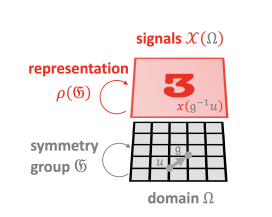
\includegraphics[width=0.5\textwidth]{geometric_deep_learning.png} % ajuster la taille
    \caption{Concept d'image} % légende
    \label{fig:mon_image} % label pour référence
\end{figure}
Soit x $\in$ $\Omega$ tel x = (i,j) avec i $\in$ X et j $\in$ Y 
Notre pixel a quatre voisins : (i+1,j) (i-1,j), (i,j-1), (i,j+1) et notre postulat principal est que les valeurs de chacun de ces points voisins (ie leur représentation dans X($\Omega$)) ne sont pas totalement décorrélées de la valeur du signal au point x. En effet, si cela était le cas, toutes nos images seraient similaires à celle-là : 
\begin{figure}[H] % h = "here", pour placer l'image ici
    \centering    % centre l'image
    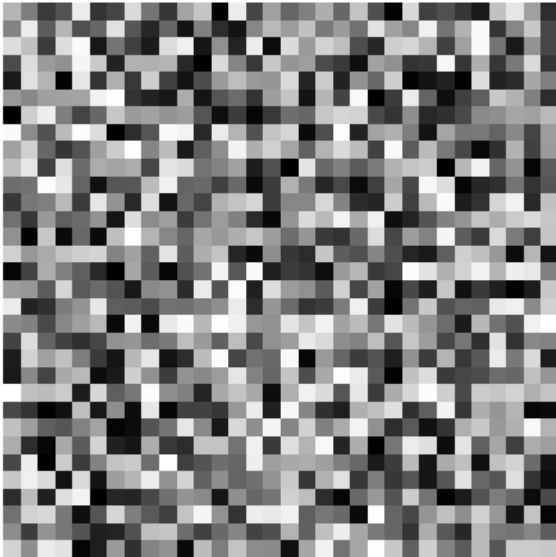
\includegraphics[width=0.4\textwidth]{random_image.png} % ajuster la taille
    \caption{Architecture d'une image} % légende
    \label{fig:mon_image} % label pour référence
\end{figure}
La performance d'un réseau de neurones est peut-être mesuré par la précision de ses prédictions mais aussi lorsqu'il s'agit de déployer le dit réseau de neurones sur un système embarqué, par la durée de l'inférence et de son poids. Ici, nous nous intéresserons en particulier, à ce troisième critère. Etant donné, un réseau de neurones CNN, comment parvenir, sans modifier sa précision a diminué sa taille ? Si la taille d'une couche linéaire est donné par le nombres de  neurones, la taille d'une couche de convolution est donné par le nombreux de filtres et leurs tailles. Ainsi, réduire la taille d'une couche de convolution signifie réduire le nombre ou la taille des filtres. Plus souvent, le nombre tant un réseaux de neurones peut compter des dizaines, centaines voir millier de couches de convolutions tandis que le kernel est de manière standard pris à 3. Ainsi, si on part du principe que diminuer la taille d'un réseau de convolution signifie d'abord diminuer son nombre de filtre, la question demeure de comment sélectionner les filtres à garder de ceux à supprimer. Plusieurs méthodes existent, les plus courantes sont les suivantes 
\\ \\ Soit $\Omega_{h}$ le domain d'un filtre $ h = (h_{i,j})_{i,j\in\Omega_h}$ avec $h_{i,j} = X_j((i,j))$ et $X_j$ signal définit sur $\Omega_h$le signal définit au coordonné au point (i,j) ou "poids" en i,j. Alors on définit : 
\\
\\
La norme L1 du filtre h :  
\[
\|h\|_1 = \sum_{i=1}^{M} \sum_{j=1}^{N} |h_{i,j}| 
\]
La norme L2 du filtre h :
% Norme L2
\[
\|h\|_2 = \sqrt{\sum_{i=1}^{M} \sum_{j=1}^{N} h_{i,j}^2}
\]
La norme infini du filtre h 

\[
\|h\|_\infty = \max_{i,j} |h_{i,j}|
\]


D'autres normes existent mais ci-dessus demeure les principales. 
Il s'agit alors d'appliquer la norme choisit sur chacun des filtres des couches de convolutions puis de choisir un seuil sur les valeurs des normes au-dessus duquel un filtre est conservé ou supprimé. 
Ces normes sont des mesures de magnitudes : elle quantifie l'importance numérique des poids. Elle suppose ainsi qu'un filtre de magnitude faible contribue peu à la sortie d'un modèle et peut donc, selon un seuil donné, être supprimé. 
Cette approche est naturel puisque qu'après, l'opération de convolution est une opération based sur la simple valeur numérique des poids. 
Hors en reposant sur un calcul de somme, ces normes sont invariantes par permutations du signal sur le filtre.

\begin{figure}[H] % h = "here", pour placer l'image ici
    \centering    % centre l'image
    
\includegraphics[width=0.5\textwidth]{dispersion_carre} % ajuster la taille
    \caption{5 filtres au hasard extrait du modèle initial entrainé} % légende
    \label{fig:mon_image} % label pour référence
\end{figure}
Les deux filtres ci-dessus bien que de motif radicalement différents sont deux normes L1,L2 et Linfini identique. 
L'objectif de cette exemple volontairement simpliste n'est pas tant de trouver des défauts au norme L1, L2 mais plutôt d'introduire une approche conceptuelle nouvelle : la régularité.
Comme mentionné en introduction, les images par la présence de motifs, forme, bords ou aux autres présentes des régulatirés. Aussi, l'objectif d'un filtre de convolution est de capturer de tels motifs en agissant comme un mask glissant sur le domaine de l'image. Ainsi, ces filtres doivent aussi témoigner de régularités. 
Cependant, s'ils existent, comment les mesures ? En effet, un filtre peut-être globalement régulier mais aussi localement régulier ou régulier localement et globalement mais selon des motifs différent. 
Tant bien même toutes ces questions, nous postulons que la magnitude d'un filtre n'est plus condition suffisante de survie dans une méthode de pruning, un filtre au-delà de sa magnitude devrait aussi être régulier. 
Par ailleurs, nous n'affirmons non plus que la régularité soit suffisante mais bien que cette deux approches doivent être complémentaires. 
\subsection{Objectif}
Notre objectif est de construire une modèle de classification à destination du dataset cifar10. Nous souhaitons en particulier, minimiser sa taille, tout en conservant une accuracy d'au moins 80 \% 
En effet, comme nous avons pu le voir précédemment le modèle VGG proposé est trop lourd pour être embarqué sur STM32. 
\subsection{Approche}
Afin de définir un modèle plus compact, nous partirons d'une architecture similaire à celle donnée initialement. Dans un premier construire une mesure de régularité. Cette mesure nous permettra de définir une méthode de pruning structurel. Méthode que nous utiliserons pour 
réduire la taille de notre modèle, dans un second temps. 
 Une fois, la mesure créée. Les étapes seront les suivantes : 
\begin{enumerate}
    \item \textbf{Entrainement du modèle }: nous récupérons le modèle initial puis nous l'entrainons afin de pouvoir récupérer les poids des filtres relativement à chaque filtres. 
    \item \textbf{Classification des filtres }: nous classifions, selon une méthode à définir, les filtres en fonction de leur régularité après le première entrainement. 
    \item \textbf{Suppression des filtres et reconstruction du modèle} : nous extrayons un pourcentage p données de filtre en fonction de la classification précédent puis reconstruisons un modèle avec ces nouveaux filtres. 
    \item \textbf{Fine Tuning du nouveau modèle} : une fois p-1 pourcentes  filtres supprimés dans le modèle initials, que réintrénons le second modèle obtenu. 
    \item \textbf{Evaluation du nouveau modèle} : nous évaluons le nouveau modèlons et comparons ses performances en terme de précision et de taille mémoire avec le modèle initial non pruné. 
\end{enumerate}
\subsection{Entrainement du modèle} 
Le postulat de départ s'appuyé sur la présence de régularité dans les poids des filtres. Pour cela, essayons de prime à bord de visualiser les poids du modèles entrainés afin d'intuiter cette hyptohèse de départ. 
\begin{figure}[H] % h = "here", pour placer l'image ici
    \centering    % centre l'image
    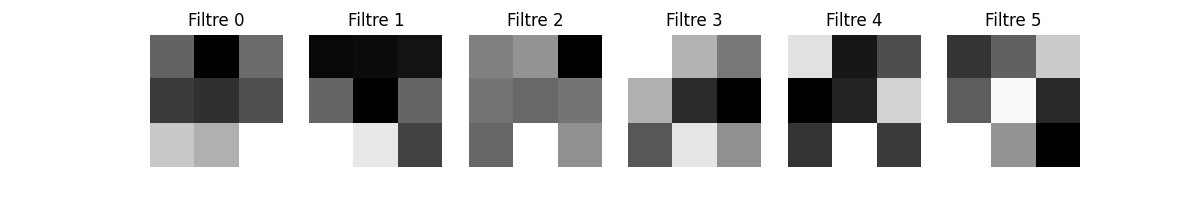
\includegraphics[width=1\textwidth]{kernel_3D_3par3.png} % ajuster la taille
    \caption{5 filtres au hasard extrait du modèle initial entrainé} % légende
    \label{fig:mon_image} % label pour référence
\end{figure}
Ici, l'on constate un problème d'échelle. Sur des kernel en dimension 3, il est difficile de distinguer un signal, une régularité, d'un bruit. La donnée des filtres n'est pas suffisament riches, pour identifier des patterns dans leurs distributions, avec si peu de données la probabilité d'interpréter un signal en bruit est élevé. Ainsi, nous ne pouvons travailler avec le modèle tel quel, nous travaillerons plutôt avec des kernels de taille 5. 
\begin{figure}[H] % h = "here", pour placer l'image ici
    \centering    % centre l'image
    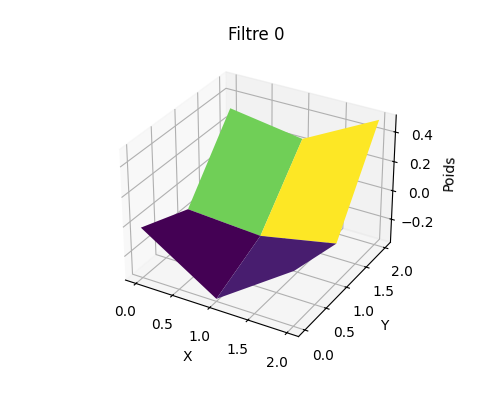
\includegraphics[width=0.4\textwidth]{kernel_3D_3par_3D.png} % ajuster la taille
    \caption{Filtre de convolution affiché en 3D : difficile d'identifier quel que pattern que ce soit. } % légende
    \label{fig:mon_image} % label pour référence
\end{figure}
En augmentant la taille des kernels, les filtres font apparaitre une topologie plus riche, proprice à l'analyse. 
\begin{figure}[H] % h = "here", pour placer l'image ici
    \centering    % centre l'image
    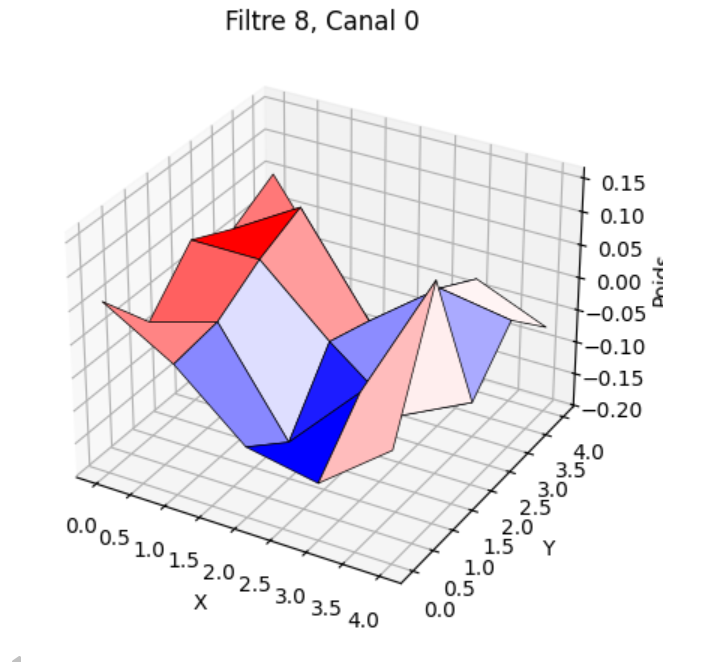
\includegraphics[width=0.4\textwidth]{filtre_3D.png} % ajuster la taille
    \caption{Filtre de convolution avec un kernel de taille 5x5 } % légende
    \label{fig:mon_image} % label pour référence
\end{figure}
Sur l'image ci-dessus, les géométrie rouges identiques des valeurs de poids positives, tandis que les géométriques bleus des valeurs de poids négatifs. De prime à bords, il parait plus simple d'identifier des points critiques. 
\subsection{Traitement des poids}

Les filtres de convolutions utilisés dans le modèle initial avec un kernel de dimension 9 (3x3), dans notre cas, afin de pouvoir établir une mesure suffisamment pertinente sur les filtres, nous augmentons la taille des kernel de 3 à 5. Cette augmentation de taille, augmente considérablement la taille du réseau de neurones. En effet, on passe de 9 à 25 paramètres par filtre. Ainsi si une couche à $c_{in}$ canaux et $c_{out}$ filtres alors la couche à $\Delta$ nouveaux paramètres  
\[ \Delta param = c_{in} * c_{out} * (25-9) \]
Ainsi pour chaque couche on obtient : 
\begin{enumerate}
    \item Conv2D(32, $3\times3$, input\_shape=(32,32,3))  
    \[
    \Delta = 16 \times 3 \times 32 = 1,536
    \]

    \item Conv2D(32, $3\times3$) (entrée = 32 canaux)  
    \[
    \Delta = 16 \times 32 \times 32 = 16,384
    \]

    \item Conv2D(64, $3\times3$) (entrée = 32 canaux)  
    \[
    \Delta = 16 \times 32 \times 64 = 32,768
    \]

    \item Conv2D(64, $3\times3$) (entrée = 64 canaux)  
    \[
    \Delta = 16 \times 64 \times 64 = 65,536
    \]

    \item Conv2D(128, $3\times3$) (entrée = 64 canaux)  
    \[
    \Delta = 16 \times 64 \times 128 = 131,072
    \]

    \item Conv2D(128, $3\times3$) (entrée = 128 canaux)  
    \[
    \Delta = 16 \times 128 \times 128 = 262,144
    \]
\end{enumerate}
Soit en tout 509,440 nouveaux paramètres. Le modèle devient alors celui-ci : 
\begin{lstlisting}[language = python]
    
       model = nn.Sequential(
        # Bloc 1
        nn.Conv2d(3, 32, kernel_size=5, padding=2),
        nn.BatchNorm2d(32),
        nn.ReLU(),
        nn.Conv2d(32, 32, kernel_size=5, padding=2),
        nn.ReLU(),
        nn.BatchNorm2d(32),
        nn.SpatialDropout2d(0.25) if hasattr(nn, 'SpatialDropout2d') else nn.Dropout2d(0.25),
        nn.MaxPool2d(2),

        # Bloc 2
        nn.Conv2d(32, 64, kernel_size=5, padding=2),
        nn.BatchNorm2d(64),
        nn.ReLU(),
        nn.Conv2d(64, 64, kernel_size=5, padding=2),
        nn.ReLU(),
        nn.BatchNorm2d(64),
        nn.SpatialDropout2d(0.25) if hasattr(nn, 'SpatialDropout2d') else nn.Dropout2d(0.25),
        nn.MaxPool2d(2),

        # Bloc 3
        nn.Conv2d(64, 128, kernel_size=5, padding=2),
        nn.BatchNorm2d(128),
        nn.ReLU(),
        nn.SpatialDropout2d(0.25) if hasattr(nn, 'SpatialDropout2d') else nn.Dropout2d(0.25),
        nn.MaxPool2d(2),

        # Bloc 4
        nn.Conv2d(128, 128, kernel_size=5, padding=2),
        nn.BatchNorm2d(128),
        nn.ReLU(),
        nn.SpatialDropout2d(0.25) if hasattr(nn, 'SpatialDropout2d') else nn.Dropout2d(0.25),
        nn.MaxPool2d(2),

        # INNOVATION: Adaptive pooling pour taille fixe
        nn.AdaptiveAvgPool2d((4, 4)),

        # Classificateur compact progressif
        nn.Flatten(),  # 128 * 4 * 4 = 2048
        nn.Linear(2048, 1024),
        nn.ReLU(),
        nn.Dropout(0.3),
        nn.Linear(1024, 512),
        nn.ReLU(),
        nn.Dropout(0.3),
        nn.Linear(512, 10)
    ).to(device)

    
\end{lstlisting}
Le modèle ainsi crée possède 3,425,450 paramètres et une taille estimé de 16,20 Mo. 
Toutefois, au délà de la taille des convolutions, augmente la taille des kernel augmente considérablement la taille et ainsi le nombre de paramètres des couches linéaires. 
En effet,dans ce nouveau modèle 77 \% des paramètres du modèles appartiennent à la couche linéaire, laquelle ne permettant que des transformations linéaires n'est pas suffisant déterminant dans l'identification des motifs pour justifier une telle répartition de poids. 
Afin de diminuer la taille initial du modèle tout en gardant un kernel size supérieur à 3. Nous allons mettre en place plusieurs changement : 
\paragraph{Réduction du kernel size de 5 à 4 }
Rappelons que dans la cadre du projet, nous voulons utiliser notre modèle sur des images de taille 32*32, un kernel size de 4 sera alors suffisant et permettrait d'abord de diminuer la taille du modèle. 
En effet, par exemple sur Conv(32→32)
\begin{itemize}
    \item Avec kernel size égale 5 : 32*32*5*5 = 25.600 paramètres
    \item Avec kernel size égale 4 : 32*32*4*4 = 16.384 paramètres
\end{itemize}
Soit une réduction effective de 36 \% des paramètres pour cette couche.
De plus, si on calcule le réceptive field (la région de l'image d'entrée qui influence un pixel de sortie), on constate que diminuer le kernel size à 4 est toujours suffisant. En effet : 
\begin{itemize}
\item Après Conv1: RF = 4
\item Après Conv2: RF = 4 + (4-1) = 7
\item Après Pool1: RF = 7 * 2 = 14
\item Après Conv3: RF = 14 + (4-1) = 17
\item Après Conv4: RF = 17 + (4-1) = 20
\item Après Pool2: RF = 20 * 2 = 40
\end{itemize}
Ainsi le RF du modèle pour kernel size de 4 est suffisant pour des images de taille 32*32. 
\paragraph{Bottleneck 1*1}
Un bottleneck est l'équivent d'une transformation linéaire mais appliqué spatialement. Plus spécifiquement, la convolution 1*1 apprend une transformation linéaire du vecteur de taille nombre de canaux pour chaque pixel du filtre où elle s'applique
En pratique, c'est simplement une couche de convolution avec un kernel size de 1. L'avantage du bottleneck réside aussi dans la réduction de paramètres. 
En effet, pour passer par exemple d'une taille de 128 à 64 canaux, une 1×1 coûte :
\begin{itemize}
   \item 1×1 : 128 * 64 * 1 * 1 = 8,192 paramètres
   \item 5×5 : 128 * 64 * 5 * 5 = 204,800 paramètres
\end{itemize}
Soit une réduction de 96 \% des paramètres dans cet exemple. 
\paragraph{AdaptativeAvgPool(1,1)}
En utilisant un AdaptativeAvgPool de taille (1,1) au lieu de (4,4) on divise ainsi par 16 la taille de sortie. Avant, utiliser une taille de 4*4 revenait à divisier la carte en 8*8 en grille 4*4 puis à garder la moyenne 
de chaque région 2*2. Avec cette modification, pour chaque canal on garde la moyenne de toute la carte spatiale. Ce changement 
permet d'ajouter une invariance par translation naturelle, qu'importe la position d'un objet donné à détecter sur l'image, l'adaptative pooling donnera des valeurs similaires. 
Ce qui permet de diminuer l'overfitting spatiale relativement aux positions des objets sur l'image. 

Nous proposons ainsi un nouveau modèle incorporant ces trois changements : 
\begin{lstlisting}[language=Python]
model = nn.Sequential(
    # Bloc 1
    nn.Conv2d(3, 32, kernel_size=4, padding=1, bias=True),
    nn.ReLU(),
    nn.BatchNorm2d(32),

    nn.Conv2d(32, 32, kernel_size=4, padding=1, bias=True),
    nn.ReLU(),
    nn.BatchNorm2d(32),
    nn.MaxPool2d(2, 2),
    nn.Dropout2d(0.2),

    # Bloc 2
    nn.Conv2d(32, 64, kernel_size=4, padding=1, bias=True),
    nn.ReLU(),
    nn.BatchNorm2d(64),

    nn.Conv2d(64, 64, kernel_size=4, padding=1, bias=True),
    nn.ReLU(),
    nn.BatchNorm2d(64),
    nn.MaxPool2d(2, 2),
    nn.Dropout2d(0.3),

    # Bloc 3
    nn.Conv2d(64, 128, kernel_size=4, padding=1, bias=True),
    nn.ReLU(),
    nn.BatchNorm2d(128),

    nn.Conv2d(128, 128, kernel_size=1, padding=0, bias=True),  # bottleneck
    nn.ReLU(),
    nn.BatchNorm2d(128),
    nn.AdaptiveAvgPool2d((1,1)),

    nn.Flatten(),

    # Classifier compact
    nn.Linear(128, 128),
    nn.ReLU(),
    nn.Dropout(0.4),
    nn.Linear(128, 10)
    ).to(device)
\end{lstlisting}

Concrêtement, nous observons l'effet directement sur la taille de nos couches linéaires. Lesquels non seulement sont moins nombreuses (3 dans l'ancien modèle et 2 dans le nouveau) mais contiennent aussi moins de paramètres. 
En effet, dans l'ancien modèle ces couches contenait 2 626 560 paramètres contre seuleument 17 664 dans la nouvelle architecture soit une réduction de 99.3 \%
Ci-dessus, l'analyse final de le notre modèle : 

\begin{lstlisting}[language=Python]
    ----------------------------------------------------------------
        Layer (type)               Output Shape         Param #
================================================================
            Conv2d-1           [-1, 32, 31, 31]           1,568
              ReLU-2           [-1, 32, 31, 31]               0
       BatchNorm2d-3           [-1, 32, 31, 31]              64
            Conv2d-4           [-1, 32, 30, 30]          16,416
              ReLU-5           [-1, 32, 30, 30]               0
       BatchNorm2d-6           [-1, 32, 30, 30]              64
         MaxPool2d-7           [-1, 32, 15, 15]               0
         Dropout2d-8           [-1, 32, 15, 15]               0
            Conv2d-9           [-1, 64, 14, 14]          32,832
             ReLU-10           [-1, 64, 14, 14]               0
      BatchNorm2d-11           [-1, 64, 14, 14]             128
           Conv2d-12           [-1, 64, 13, 13]          65,600
             ReLU-13           [-1, 64, 13, 13]               0
      BatchNorm2d-14           [-1, 64, 13, 13]             128
        MaxPool2d-15             [-1, 64, 6, 6]               0
        Dropout2d-16             [-1, 64, 6, 6]               0
           Conv2d-17            [-1, 128, 5, 5]         131,200
             ReLU-18            [-1, 128, 5, 5]               0
      BatchNorm2d-19            [-1, 128, 5, 5]             256
           Conv2d-20            [-1, 128, 5, 5]          16,512
             ReLU-21            [-1, 128, 5, 5]               0
      BatchNorm2d-22            [-1, 128, 5, 5]             256
AdaptiveAvgPool2d-23            [-1, 128, 1, 1]               0
          Flatten-24                  [-1, 128]               0
           Linear-25                  [-1, 128]          16,512
             ReLU-26                  [-1, 128]               0
          Dropout-27                  [-1, 128]               0
           Linear-28                   [-1, 10]           1,290
================================================================
Total params: 282,826
Trainable params: 282,826
Non-trainable params: 0
----------------------------------------------------------------
Input size (MB): 0.01
Forward/backward pass size (MB): 2.19
Params size (MB): 1.08
Estimated Total Size (MB): 3.28
----------------------------------------------------------------
\end{lstlisting}
En particulier, nous constatons que ce nouveau modèle pèse 3.28 Mb contre 16.2 Mb pour l'ancien, lequel contenait 3.4 millions de paramètres contre 282 mille paramètres pour la nouvelle architecture.
\subsubsection{Analyse des poids post-entrainement}

Maintenant que nous avons augmenté la taille des kernels tout en gardant une taille résonable,  nous entraînons afin de pouvoir examiner les poids de notre nouveau modèle.
L'entrainement est réalisé avec une fonction de perte CrossEntropyLoss, l'optimiseur Adam, le tout avec 30 epochs. Nous chargons les données d'entrainement avec un bootloader de batchsize 32 et normalisons les poids des entrées en divisant toutes les valeurs des pixels des images par 255. 
Les résultats de l'entrainement sont les suivants : 
\begin{figure}[H] % h = "here", pour placer l'image ici
    \centering    % centre l'image
    \includegraphics[width=1\textwidth]{training_new_modele.png} % ajuster la taille
    \caption{Résultat d'entrainement du modèle sur 30 epochs } % légende
    \label{fig:mon_image} % label pour référence
\end{figure}
A la fin de l'entrainement, cette version augmentée du modèle initial est aussi précise que le modèle VGG16 et déjà inférieure à 5Mo. L'absence d'oscillation confirme le choix du batch size, du taux d'apprentissage, des paramètres dont la mauvaise calibration tend à créer du bruit statistique sur les courbes de loss et d'accuracy. 
\begin{figure}[H] % h = "here", pour placer l'image ici
    \centering    % centre l'image
    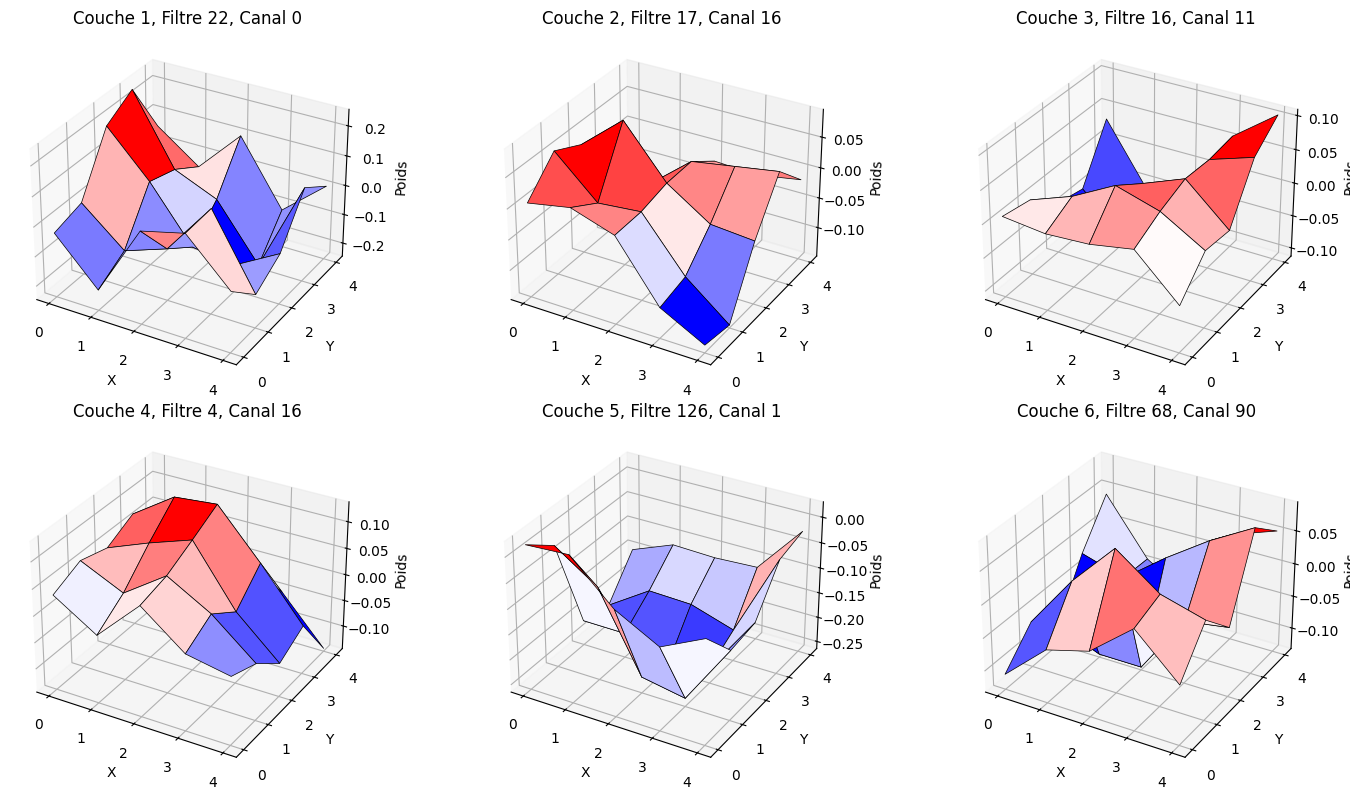
\includegraphics[width=0.9\textwidth]{filtre_3D_modele.png} % ajuster la taille
    \caption{Poids de 6 filtres tirés au hasard dans 6 couches de convolutions différentes} % légende
    \label{fig:mon_image} % label pour référence
\end{figure}
Cette augmentation de kernel, nous permet à présent de travailler de travailler dans un sous ensemble de $\mathbb{R}^{16}$ Ce qui nous permet non pas de voir des géométries plus fines dans la distribution des poids mais d'avoir une vue plus global ce qui à termes nous d'identifier des régularités à différentes échelles dans les filtre. En effet, la suppression d'un filtre doit se faire tant sur l'absence de signal sur l'ensemble de ses poids, que l'absence de signal dans des sous-ensembles de l'ensemble de ses poids. 
Ci-dessous, un figuré présentant une première ligne de filtres dont les valeurs des poids sont aléatoires puis une seconde rangée possèdent une partie de leurs filtres avec des valeurs aléatoires et une seconde suivant une gausienne. Nous cherchons ainsi à établir une méthode nous permettant de distinguer à la fois des filtres ne présentant pas de signal globalement, tout comme ne présentant pas de signal localement, tout comme ne présentant pas de signal du tout. 
\begin{figure}[H] % h = "here", pour placer l'image ici
    \centering    % centre l'image
    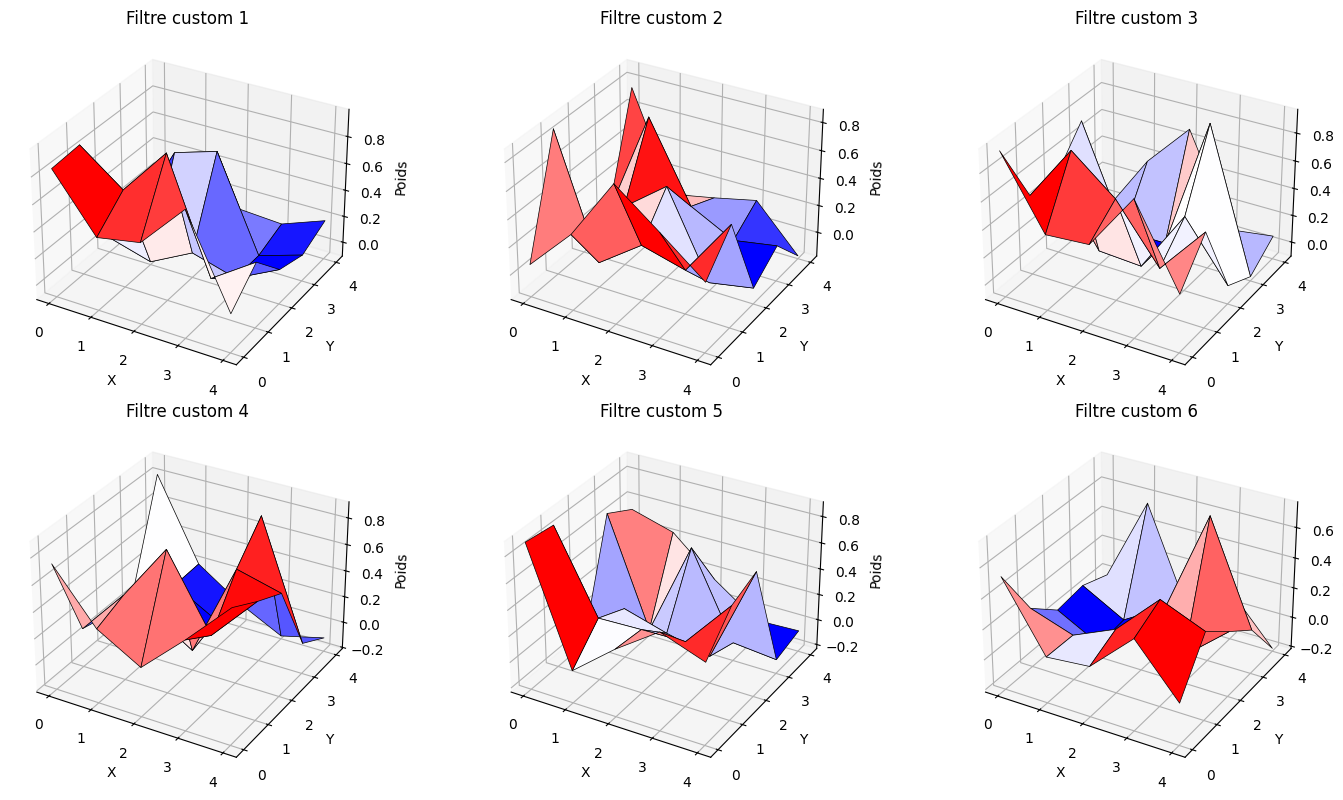
\includegraphics[width=0.9\textwidth]{mixte_distribution.png} % ajuster la taille
    \caption{Poids de 6 filtres tirés au hasard dans 6 couches de convolutions différentes} % légende
    \label{fig:mon_image} % label pour référence
\end{figure}
L'aspect multi-échelle de notre analyse est au coeur de notre approche car c'est bien des régularités d'échelles (ie taille) différentes qui seront détecter par nos filtres. Un filtre aux valeurs en apparrence irrégulière pouvant ainsi être assimilé à un filtre ayant échoué à détecter quelqueconque pattern à quelconque échelle.

Bien qu'une taille de kernel 4x4 facilite notre analyse, cela ne demeure toujours pas suffisant pour nos outils d'analyses. Or nous ne pouvant nous permettre non plus d'augmenter encore la taille du kernel, nous allons donc projeter artificiellement notre espace de dimension 25 dans un espace de dimension encore plus grand, continue, l'espace de Schwartz $S(\mathbb{R}^2)$
Projeter revient à faire une interpolation des poids de notre filtre par une fonction d'un espace donné, ici l'espace de Schwartz.
\subsubsection{Projection dans un espace continue : l'espace de Schwartz $S(\mathbb{R}^2)$}
\subparagraph{Définition}
Une fonction $f : \mathbb{R}^2 \to \mathbb{R}$ est dite \emph{à décroissance rapide} si elle est infiniment dérivable et si, pour tout couple d'entiers $m,n \ge 0$, il existe une constante $C_{m,n} > 0$ telle que
\[
\forall (x,y) \in \mathbb{R}^2.\quad
|x^m y^n f(x,y)| \le C_{m,n},
\]

Autrement dit, $f$ et toutes ses dérivées décroissent plus vite que n'importe quelle puissance négative de $|x|$ et $|y|$ lorsque $(x,y)$ tend vers l'infini.  

On appelle alors $S(\mathbb{R}^2)$ (espace de Schwartz) l'espace vectoriel des fonctions de $\mathbb{R}^2$ dans $\mathbb{C}$ qui vérifient les deux conditions suivantes : 
\begin{itemize}
    \item f est $\mathbb{C^{\infty}}$
    \item f et toutes ses dérivées sont à décroissantes rapide. 
\end{itemize}
\subparagraph{Usage}
Dans notre cas, nous travaillons en faite pas directement dans l'espace de Schwartz qui est à valeur dans $\mathbb{C}$ mais dans un sous espace de Schwartz à valeur réelle.
Travaillé dans $S(\mathbb{R}^2)$ permet plusieurs choses : 
\begin{enumerate}
    \item C'est un espace de fonction très régulière et de convergence rapide, permettant d'éviter d'éventuels effets de bord sur les abords du filtres ou singularité dans la distribution
    \item Pour notre analyse, nous souhaitons utiliser la transformée de Fourier laquelle se comporte bien dans cette espace. En effet, l'espace est stable par transformée de Fourier, donc pas de divergence possible ou création d'artefacts lors de l'application de la transformée de Fourier, le filtre restera lisse.
       
\end{enumerate}
\subparagraph{Construction}
Pour simuler un tel espace, nous allons procéder en trois temps. 
D'abord, il s'agit de définir le filtre comme une fonction continue : 

\[
F : [0, H-1] \times [0, W-1] \to \mathbb{R}
\]
telle qu'elle coïncide avec les valeurs discrètes sur la grille :
\[
\forall (n,m) \in \Omega \quad F(n,m) = h[n,m]
\]
Entre les points de la grille, F est lisse, ie $F \in C^2([0,H-1] \times [0,W-1])$ 
On utilise ensuite l’interpolateur cubique bilinéaire lequel minimise une énergie de lissage quadratique locale afin de déterminer F en dehors de ces points.
F réalise le min suivant : 

\[
\min_{F \in C^2} (\sum_{n,m} \left| F(n,m) - h[n,m] \right|^2 
+ \lambda \iint \Bigg( 
\left(\frac{\partial^2 F}{\partial x^2}\right)^2 
+ 2 \left(\frac{\partial^2 F}{\partial x \partial y}\right)^2 
+ \left(\frac{\partial^2 F}{\partial y^2}\right)^2 
\Bigg) \, dx\, dy)
\]
On redéfinit ensuite grille fine $(y_i, x_j)$ avec 
$i,j = 0, \dots, S-1$ pour un S un "smooth operator" :

\[
y_i = \frac{i(H-1)}{S-1}, \quad x_j = \frac{j(W-1)}{S-1}, \quad i,j = 0,\dots,S-1
\]

et on construit la matrice de valeurs interpolées :

\[
Z_{\text{smooth}}[i,j] = F(y_i, x_j), \quad i,j = 0,\dots,S-1
\]
Toutefois, nous n'avons pas encore tout à fait généré notre espace de Schwartz, il faut pour cela multiplie notre fonction par un facteur garantissant non seulement la régularité mais aussi la stabilité de notre ensemble. Naturellement, on utilisera une fenetre gausienne : 

On peut multiplier par une fenêtre gaussienne centrée sur le filtre. 

\[
F_S(y_i,x_j) = Z_{smooth}[i,j] \cdot \exp\Bigg( - \frac{(y_i - H/2)^2 + (x_i - W/2)^2}{2\sigma^2} \Bigg)
\]

où $\sigma$ contrôle la décroissance de la gaussienne. Ce qui nous permet de contrôler la continuité et décroissante rapide. 
\subparagraph{Simulation} 


\begin{figure}[H] % h = "here", pour placer l'image ici
    \centering    % centre l'image
    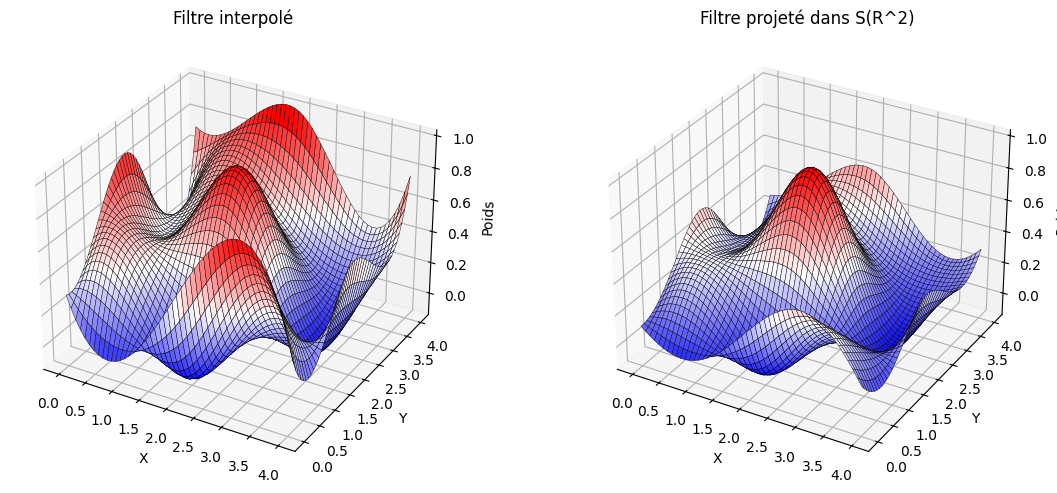
\includegraphics[width=0.7\textwidth]{projection_dans_S_aleatoire.png} % ajuster la taille
    \caption{Projection dans l'espace de Schwartz d'un filtre aléatoire} % légende
    \label{fig:mon_image} % label pour référence
\end{figure}
\begin{figure}[H] % h = "here", pour placer l'image ici
    \centering    % centre l'image
    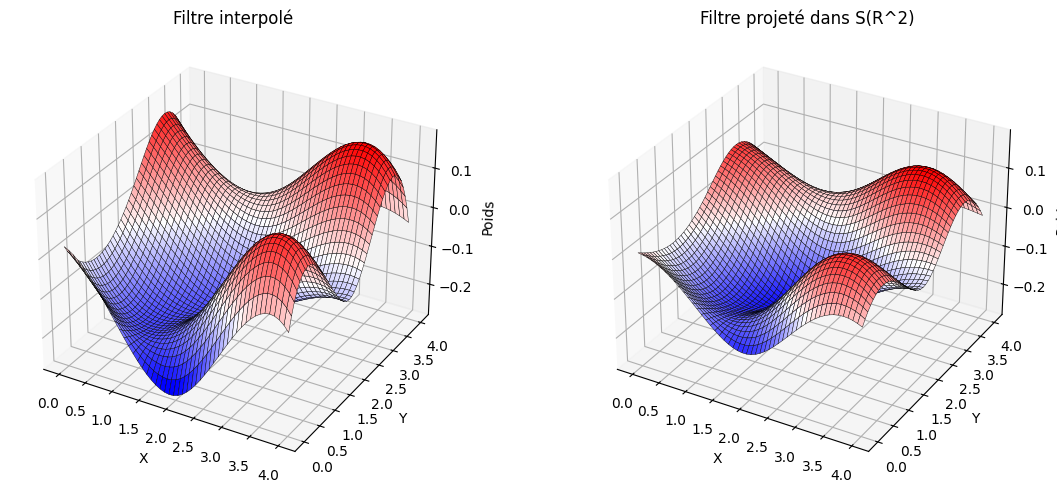
\includegraphics[width=0.7\textwidth]{projection_dans_S_modele.png} % ajuster la taille
    \caption{Projection dans l'espace de Schwartz d'un filtre du modèle entrainé} % légende
    \label{fig:mon_image} % label pour référence
\end{figure}
Sur les deux exemples, ci-dessus, on constate l'effet de "lissage" de la projection. En particulier, pour le filtre aléatoire, moins régulier.
Le code en annexe reprend successivement les deux étapes de constructions précédentes de la projection des filtres ci-dessus. 
\paragraph{Zero-padding}
Afin d'affiner notre analyse fréquentielle avec la transformée de Fourier, il faut zéro padder le filtre obtenu. Cela nous permettra d'éviter les effets de bord notamment. Aucune nouvelle information fréquentielle n’est créée (on ne change pas le support fréquentiel effectif), mais la grille d’échantillonnage fréquentiel sera plus raffermie. Soit un filtre $h$ de taille $H\times W$.  
On définit une version zéro-paddée $\tilde{h}$ sur une grille plus grande $H' \times W'$ (avec $H' \geq H,\ W' \geq W$) :

\[
\forall (n,m)\in H' \times W' \quad 
\tilde{h}[n,m] =
\begin{cases}
h[n,m], & 0 \leq n < H,\ 0 \leq m < W \\
0, & \text{sinon}.
\end{cases}
\]

\subsubsection{Mesure de régularité}
Maintenant que le cadre d'analyse est posé, nous allons définir notre mesure de régularité. Nous cherchons à analyser la présence de régularité dans nos filtres. En particulier la présence de régularités dans tous sous ensemble d'un même filtre. La transformée de Fourier permet de passer dans domaine spatial à un domaine fréquentiel permettant de considérer une fonction donnée en une somme d'ondes pures, fournissant ainsi une analyse spectrale de la régularité. Cette analyse spectrale va nous permettre de distinguer signaux forts de signaux faibles autrement dit des régularités de ce qui n'en est pas.  C'est donc naturellement qu'elle constitue l'outil principale de notre étude. En particulier, elle présente plusieurs propriété utile à notre démarche que nous allons détailler. 
\paragraph{Définition}
\subparagraph{Transformée de Fourier}
Soit $F : \mathbb{R}^2 \to \mathbb{R}$ une fonction de Schwartz, 
$F \in \mathcal{S}(\mathbb{R}^2)$.  
Sa transformée de Fourier (unités $2\pi$ comme ci-dessous) est définie par

\[
\widehat{F}(\xi) = \iint_{\mathbb{R}^2} F(x)\, e^{-2\pi i \langle x, \xi \rangle}\, dx,
\quad \xi = (\xi_1, \xi_2).
\]
\subparagraph{Théorème de Plancherel}

Si $F \in L^2(\mathbb{R}^d)$, alors sa transformée de Fourier $\widehat{f}$ est aussi dans 
$L^2(\mathbb{R}^d)$, et on a l’égalité d’énergie :

\[
\|f\|_{L^2(\mathbb{R}^d)}^2 
= \int_{\mathbb{R}^d} |f(x)|^2 \, dx
= \int_{\mathbb{R}^d} |\widehat{f}(\xi)|^2 \, d\xi
= \|\widehat{f}\|_{L^2(\mathbb{R}^d)}^2.
\]

Le théorème de Plancherel est crucial dans notre cas, en effet il garantit que travailler dans le domaine spatial ou dans le domaine fréquentiel est strictement équivalent en norme L2. Autrement dit, passer en domaine fréquentiel en appliquant la transformée de Fourier est une construction équivalente du point de vue de la magnitude. C'est important dans notre cas, car après tout, comme mentionné précédemment l'approche par régularité et par magnitude doivent être complémentaire. Appliquer la transformer de Fourier, conserve donc l'intégrité des poids selon la norme L2.   

\subparagraph{Espace de Sobolev}
Si la transformée de Fourier est utile pour notre analyse, elle ne fait pas tout ! En particulier, elle n'est pas une norme. Cependant, on peut en définir une par extension sur un espace particulier, l'espace de Sobolev. 
\subparagraph{Espace de Sobolev}
Soit $\Omega \subset \mathbb{R}^d$ un ouvert.

Pour un entier $k \in \mathbb{N}$, l’espace de Sobolev $H^k(\Omega)$ est défini comme l’ensemble des fonctions 
$f \in L^2(\Omega)$ dont toutes les dérivées jusqu’à l’ordre $k$ appartiennent aussi à $L^2(\Omega)$ :

\[
H^k(\Omega) = \bigl\{ f \in L^2(\Omega) : \partial^\alpha f \in L^2(\Omega),\ \ |\alpha| \leq k \bigr\},
\]
où $\alpha = (\alpha_1,\dots,\alpha_d)$ est un multi-indice.

La norme associée est alors :
\[
\|f\|_{H^k(\Omega)}^2 
= \sum_{|\alpha|\leq k} \|\partial^\alpha f\|_{L^2(\Omega)}^2.
\]

Pour $s \in \mathbb{R}$, pas nécessairement entier, on définit ainsi $H^s(\mathbb{R}^2)$ par transformée de Fourier :

\[
H^s(\mathbb{R}^2) = \left\{ f \in L^2(\Omega) : 
\int_{\mathbb{R}^2} (|\xi|^2)^k |\hat{f}(\xi)|^2 \, d\xi < \infty \right\}.
\] 

La norme correspondante étant alors:

\[
\|f\|_{H^s}^2 = \int_{\mathbb{R}^d} (|\xi|^2)^s |\hat{f}(\xi)|^2 \, d\xi.
\]
Ce résultat est une application directe du théorème de Plancherel et que pour tout n $\in \mathbb{N}$ \[
\widehat{f^{(n)}}(\xi) = (2 i \pi \xi)^n \, \hat{f}(\xi)
\]
 Le terme $(|\xi|^2)^s$ pondère le spectre en donnant plus d'importance 
aux hautes fréquences lorsque $s$ est grand. Définition des hautes fréquences du image ??  

\begin{itemize}
    \item Si $\hat{f}(\xi)$ décroît rapidement, l'intégrale reste finie même pour $s$ grand, 
    ce qui correspond à une fonction très régulière.
    \item Si $\hat{f}(\xi)$ décroît lentement, seuls les petits $s$ sont permis, 
    ce qui correspond à une fonction rugueuse.
\end{itemize}
En fait, plus $s$ est grand, plus $f$ est régulière; un $s$ élevé impliquant un controle fort des hautes fréquences. 
Aussi, en ce qui concerne le choix de la valeur s, on sollicite le théorème d’injection de Sobolev lequel implique : 

\[
f \in H^s(\mathbb{R}^d), \quad s > \frac{d}{2} \;\; \Longrightarrow \;\; f \text{ est continue}.
\]

On prendra donc le s le plus petit possible (pour limiter la perte d'information dans les hautes fréquénces) vérifiant cette condition autrement dit s = 2
Ainsi on définit la mesure de localité : 

\[
\|f\|_{H^2}^2 = \int_{\mathbb{R}^d} (s^2+l^2)^2 |\hat{f}(\xi)|^2 \, d\xi.
\]
On approxime cette norme sur notre filtre discret par : 
\[
\|\widetilde{h}\|_{H^2}^2 \;\approx\; 
\sum_{k,\ell} \bigl(k^2 + \ell^2 \bigr)^2 \, \bigl| \widetilde{H}[k,\ell] \bigr|^2
\]

Avec l'approximation discrète de la transformée de Fourier sur notre filtre zero-padded : 
\[
\widetilde{H}[k,\ell] 
= \sum_{n=0}^{N'-1} \sum_{m=0}^{M'-1} 
\widetilde{h}[n,m] \, 
e^{-2 \pi i \left( \tfrac{k n}{H'} + \tfrac{\ell m}{W'} \right)} .
\]

Cette norme va pouvoir nous donner une estimation de la "régularité" ou rugosité de la fonction de $\mathbb{R}^2$ que nous avons définit. 
Plus la valeur de la norme est éleve, plus le filtre est irrégulier. 
Regardons sur l'exemple suivant : 
\begin{figure}[H]
\centering
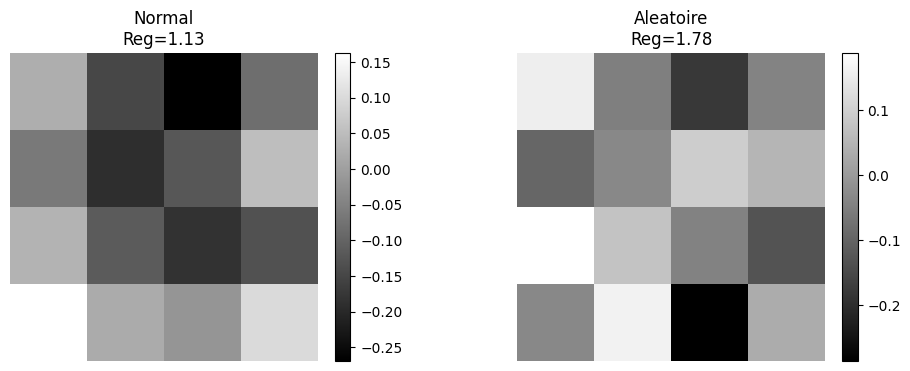
\includegraphics[width=0.8\textwidth]{test_regularite.png} % ajuster la taille
    \caption{Application de la norme de Sobolev à un filtre extrait du modèle et un filtre aléatoire} % légende
    \label{fig:mon_image} % label pour référence
\end{figure}
Sur l'exemple, ci-dessus nous observons que la mesure de Sobolev est plus faible pour le filtre extrait de notre modèle. 
A présent observons, l'effet de la projection. Rappelons-nous que la projection dépend d'un critère $\sigma$, nous allons donc tirer 100 filtres aléatoires et comparé la valeur de leurs régularité pour un filtre extrait de notre modèle de même amplitude et ceux pour deux valeurs de $\sigma = 50$ $\sigma = 1$
\begin{figure}[H] % h = "here", pour placer l'image ici
    \centering    % centre l'image
    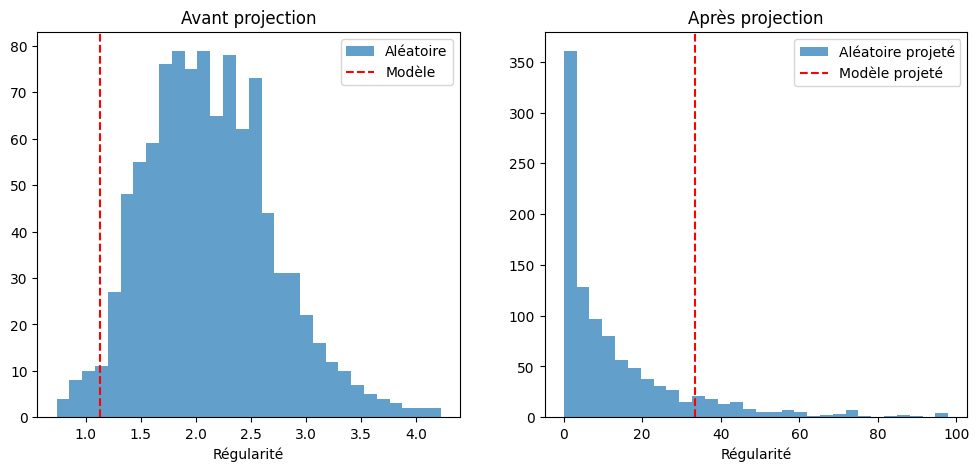
\includegraphics[width=0.8\textwidth]{test_regularite_sigma_1.png} % ajuster la taille
    \caption{Test de régularité pour une projection de valeur sigma égale 1} % légende
    \label{fig:mon_image} % label pour référence
\end{figure}
\begin{figure}[H] % h = "here", pour placer l'image ici
    \centering    % centre l'image
    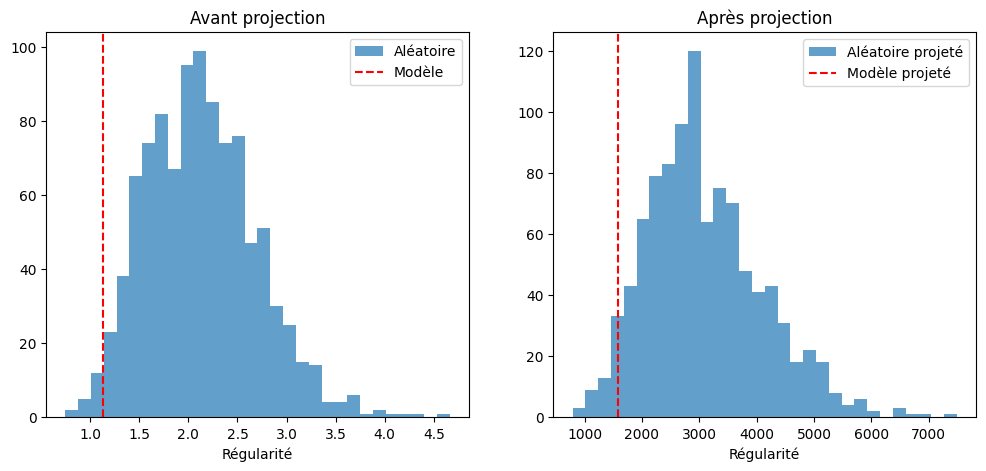
\includegraphics[width=0.8\textwidth]{test_regularite_sigma_50.png} % ajuster la taille
    \caption{Test de régularité pour une projection de valeur sigma égale 50} % légende
    \label{fig:mon_image} % label pour référence
\end{figure}
Plus la valeur de $\sigma$ est petite, plus la distribution des poids est uniformisés et concentration forte en 0. Concentration brouillant la mesure qui ne permet de faire de distinction dans la régularité. 
Au contraire pour $\sigma = 50 $ la distribution uniforme des poids semble conservé. Nous étudierons plus en détails l'effet de la variable $\sigma$ plus tard dans l'étude. 
La projection ne semble pas améliorer la distinction entre les poids réguliers des poids réguliers, mais ce à priori pour l'instant. En effet, cette mesure ne permet que de quantifier la régularité globale du filtre et non sa régularité locale. En effet, prenons l'exemple suivant : 
\begin{figure}[H] % h = "here", pour placer l'image ici
    \centering    % centre l'image
    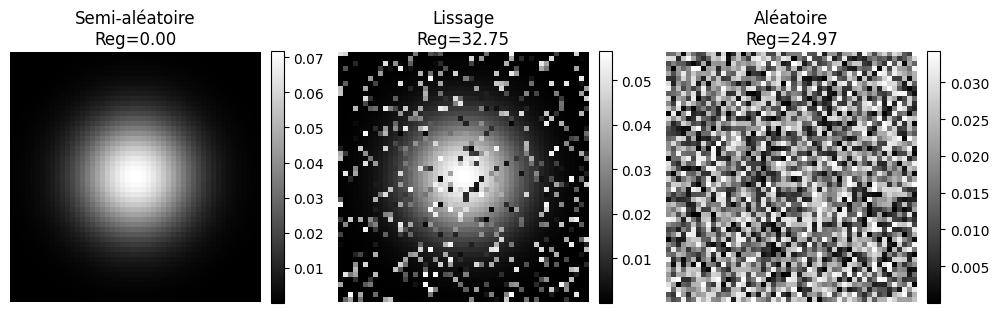
\includegraphics[width=0.8\textwidth]{importance_local.png} % ajuster la taille
    \caption{Application de la norme de Sobelev} % légende
    \label{fig:mon_image} % label pour référence
\end{figure}
Ci-dessus trois-filtre. Un premier filtre suivant une gausienne, un second une gausienne avec 20 pourcents de valeurs aléatoire et un troisième filtre totalement aléatoire. Nous pouvons constater que selon la norme établie, le second filtre bien que suivant visiblement une gausienne serait moins régulier qu'un filtre totelement  aléatoire ! En effet, la norme telle que définit ne mesure que la régularité globale, en moyennemeant les variations sur tout l'espace.  Il nous faut donc définir une mesure locale permettant de refléter la présence de régularité dans des sous-ensemble du filtre. 
\paragraph{Mesure local}
\subparagraph{Transformer de fourier fenêtré}
Afin de parvenir à capturer l'information locale de régularité, nous utilisons une transformée de fourier à fenètre glissante : 


La transformée de Fourier à fenêtre (STFT) est :

\[
V_g F(x, \xi) = \int_{\mathbb{R}^2} f(\lambda) \, \overline{g(\lambda-x)} \, e^{-2\pi i \, \xi \cdot \lambda} \, d\lambda,
\]
Avec une fenêtre 
$g \in S(\mathbb{R}^d)$.
Puis ensuite la norme de Sobolev fenetré : 
\[
\|h\|_{H^2_{\mathrm{loc}}}^2 = \int_{\mathbb{R}^2} \int_{\mathbb{R}^2} (|\xi|^2)^s \, |V_g h(x, \xi)|^2 \, d\xi \, dx
\]

Concrètement cela nous donne une indication sur ce qui se passe autour de l'absise x pour la fréquence $\lambda$
Le résultat est une mesure multi-résolution : on peut voir la régularité zone par zone. Toutefois, demeure la question du choix de la fenetre. 
\subparagraph{Choix de la fenêtre}
Nous cherchons une fonction régulière centrée autour de l'origine. Une fenêtre rectangulaire n'est pas un bon choix du fait de la discontinuité au bord et de l'effet de Gibbs qu'elle induit (apparition de déformation du signal à l'approche d'une discontinuité).

\begin{figure}[H] % h = "here", pour placer l'image ici
    \centering    % centre l'image
    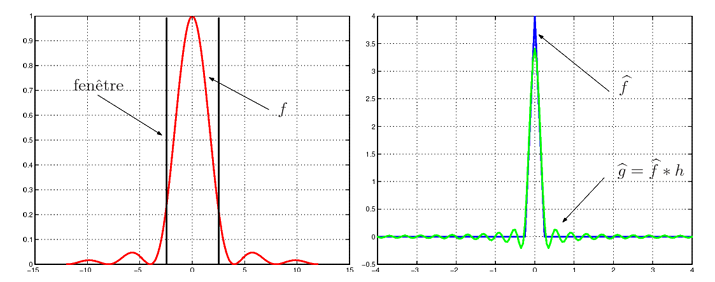
\includegraphics[width=0.8\textwidth]{Gibbs.png} % ajuster la taille
    \caption{Illustration de l'effet de Gibbs sur la fonction : $f : x \longrightarrow  \operatorname{sinc}^2( \frac{1}{4}x \pi) $, au bord du support de la fonction f apparition d'oscillation} % légende
    \label{fig:mon_image} % label pour référence
\end{figure}
Ci-dessus au abord du support la transformée de Fourier de la fonction f est multiplié par une seconde fonction : sinus cardinal. 
Cet effet est commun à tout tentative de fenetrage par une fenetre rectangulaire et découle de la propriété suivante :  pour a,b quelconques

\[
\mathcal{F}\Big(f \, \mathbf{\hat{1}}_{[a, b]}\Big) = \hat{f} * \Big(\mathbf{\hat{1}}_{[a,b]}\Big)
\]

Or $\mathbf{\hat{1}}_{[a,b]}$ est la fonction sinus cardinal, d'où le phénomène. Concernant le choix de notre fonction de fenetrage
plusieurs critères vont nous orienter vers d'éventuels candidats : 
\begin{itemize}
    \item Symétrie spectrale : la pondération spectrale ne favorise pas un sens de rotation dans le spectre. En effet, nous travaillons sur le cercle trigonométrique complexe donc le sens importe. 
    \item Conservation de l'énergie : en utilisant une fenêtre l'énergie du spectre ie la norme $L^2$ totale est inchangé
\end{itemize}
Ces deux hypothèse nous ammène à chercher d'une part une fonction paire et d'autre part de norme $L^2$ = 1. 
\begin{center}
\begin{tikzpicture}
  \begin{axis}[
    xlabel={$x$},
    ylabel={$y$},
    zlabel={$z$},
    domain=-3:3,
    y domain=-3:3,
    samples=50,
    samples y=50,
    colormap/viridis,
    view={60}{30}, % angle de vue
    width=10cm,
    height=8cm
  ]
    % Surface gaussienne
    \addplot3[surf] {exp(-0.5*(x^2 + y^2))};

    % Axe vertical en (0,0)
    
  \end{axis}
\end{tikzpicture}
\end{center}
On définit ainsi notre fenetre gausienne centré avec : 
\[
g[n,m] = \exp\Big(-2\sigma^2 \big((n-n_0)^2 + (m-m_0)^2\big)\Big), \quad n,m \in \mathbb{Z}, \quad
\sum_{n,m} g[n,m]^2 = 1
\]
A présent, appliquons cette mesure locale sur deux exmples, un filtre extrait de notre modèle entrainé et un filtre aléatoire. 
\begin{figure}[H] % h = "here", pour placer l'image ici
    \centering    % centre l'image
    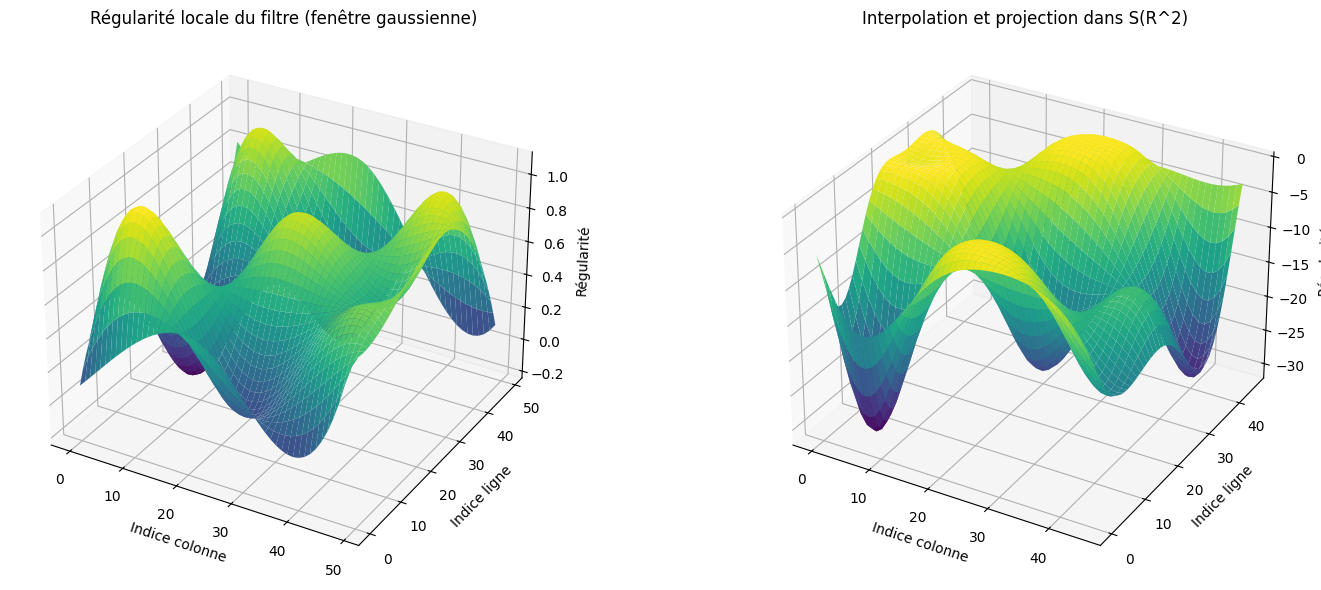
\includegraphics[width=0.8\textwidth]{application_norme_filtre_aleatoire.png} % ajuster la taille
    \caption{Application de la norme de Sobolev fenetré sur un filtre aléatoire} % légende
    \label{fig:mon_image} % label pour référence
\end{figure}
\begin{figure}[H] % h = "here", pour placer l'image ici
    \centering    % centre l'image
    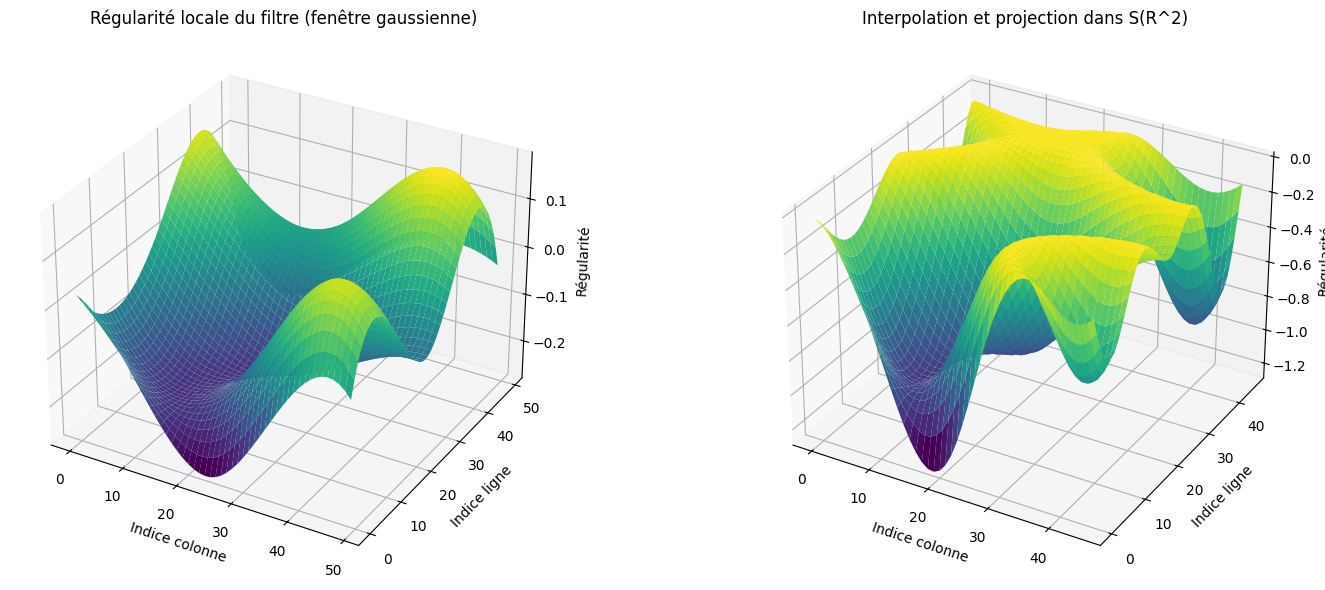
\includegraphics[width=0.8\textwidth]{application_norme_filtre_modele.png} % ajuster la taille
    \caption{Application de la norme de Sobolev fenetré sur un filtre extrait du modèle entraîné} % légende
    \label{fig:mon_image} % label pour référence
\end{figure}
Nous pouvons constater sur les deux exemples ci-dessus que notre mesure permet de distinguer, ici visuellement, un filtre aléatoire d'un filtre régulier. En effet, la map de régularité du filtre extrait du modèle est globalement localement plus proche de zero que ne l'est globalement localement le filtre aléatoire. Observons bien la différence d'échelle entre nos deux représentations de régularités !
Afin d'unifier les representations de régularités des filtres, nous les comparons par la somme de la valeur absolue des valeurs de régularités. Nous pourrions, définir des méthodes moins naives de comparaison en comparants mediane, variance etc. mais cela sort du cadre de ce rapport.
Pour le filtre régulier cette somme vaut : 714 et pour le filtre non régulier est 23374. 
\\
Si l'on reprend l'exemple précédent illustrant la nécessité d'une mesure locale. La mesure de régularité donne pour la gausienne brouillé une régularité de 8264 bien inférieur à 23374 obtenue pour le filtre totalement aléatoire, tandis que la mesure globale donnait une valeur supérieur à celle de la matrice aléatoire signifiant ainsi quelle serait moins régulière
\paragraph{Choix des paramètres de la mesure de régularité : $\sigma$}
La définition de cette mesure, nous permet aussi de revenir le choix de $\sigma$ que nous avons utilisé pour la projection dans l'espace de Schwartz. Pour rappel, pour la projection dans l'espace de Schwartz, nous avions utilisé une fenetre gausienne, laquelle permettait en lisser notre distribution et bénéficier ainsi des avantages liés à cette espace particulier notamment dans l'application de la transformée de Fourier. 
Jusqu'à présent nous utilisions $\sigma = 25$, mais est-ce une bonne valeur ? "Bonne valeur" au sens que cette dernière permettent d'un côté de lisser les courbes de poids sans pour autant supprimer les informations de régularités ou d'irrégularité en lissant trop les irrégularités de même que les évidentes régularités. La présence de bruit permet en effet aussi de remarquer la présence de signaux, cette opération de lissage doit donc être dosée. 
Plus petite la valeur de $\sigma$, plus lisse sera la distribution, nous cherchons ainsi la plus petite valeur de $\sigma$ maximisant la différent entre la valeur de régularité pour un filtre aléatoire et un filtre régulier. 
Pour cela, nous allons extraitre un nombre constant de filtre du modèle entrainé ainsi qu'un nombre constant de filtre aléatoire et pour chaque filtre caculé la valeur de la norme pour différentes valeurs de sigma. 
\begin{figure}[H] % h = "here", pour placer l'image ici
    \centering    % centre l'image
    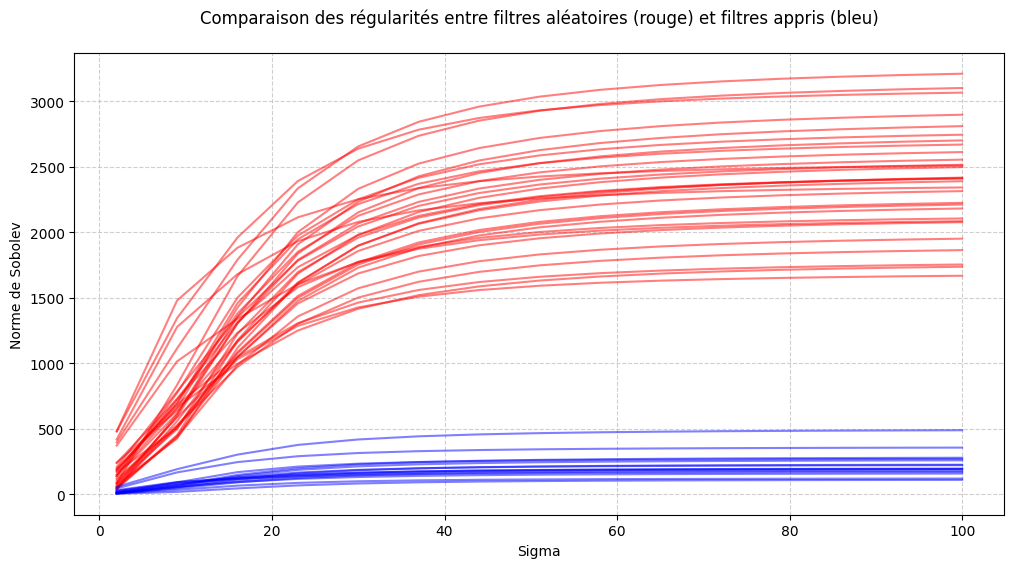
\includegraphics[width=0.6\textwidth]{regularite_aleatoire_modele.png} % ajuster la taille
    \caption{Application de la somme de la norme de Sobolev fenetré sur 10 filtres du modèles et 10 filtres instanciés aléatoirement} % légende
    \label{fig:mon_image} % label pour référence
\end{figure}
Tout d'abord, constatons sur ce premier graphique, que les filtres utilisés dans le modèle semble, au sens de cette norme, être significativement plus régulier que les filtres aleatoires. Aussi, l'on constate que que cette différence s'amenue à mesure de la valeur de sigma est petite. Enfin, nous constatons que la valeur de régularité plafonne à partir de sigma = 60. Plus précisement, la valeur est maximal à plus ou moins 5 \% à partir de sigma = 58.  
\begin{figure}[H] % h = "here", pour placer l'image ici
    \centering    % centre l'image
    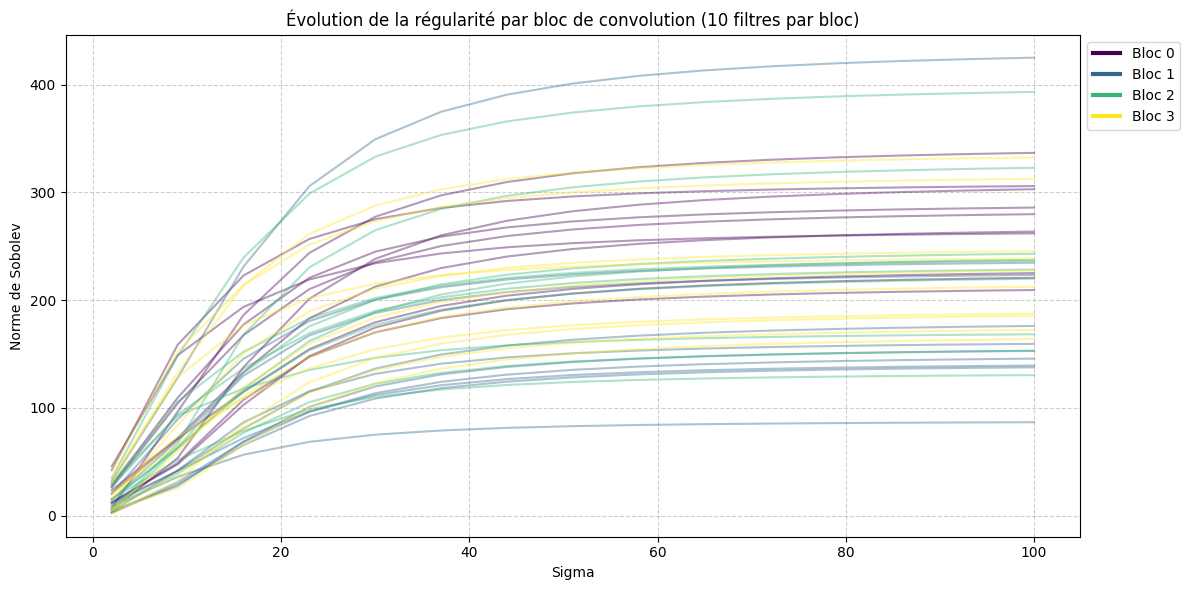
\includegraphics[width=0.6\textwidth]{regularite_par_bloc.png} % ajuster la taille
    \caption{Application de la somme de la norme de Sobolev fenetré sur 10 filtres choisies aleatoirement dans chaque bloc de convolution} % légende
    \label{fig:mon_image} % label pour référence
\end{figure}
Plus particulièrement, nous retrouvons cette évolution caractéristique au sein des filtres du modèle entrainé. 
\begin{figure}[H] % h = "here", pour placer l'image ici
    \centering    % centre l'image
    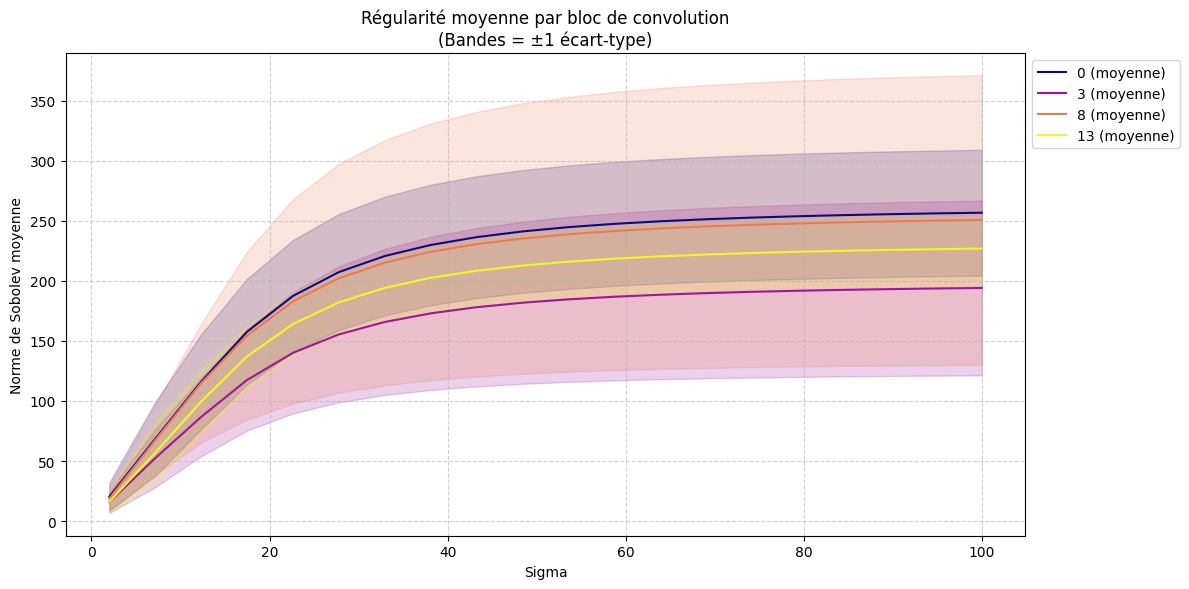
\includegraphics[width=0.6\textwidth]{regularite_moyenne_par__bloc.png} % ajuster la taille
    \caption{Moyenne de la somme de la norme de Sobolev par bloc} % légende
    \label{fig:mon_image} % label pour référence
\end{figure}
Plus globalement, en moyennement la valeur des filtres par bloc de convolution, nous observons que le niveau de profondeur du bloc de convolution, ne semble pas, à première vue en tout cas, être déterminant dans la régularité des filtres. 
Similairement la valeur d'écart type par filtre ne semblent ne nous permet pas de conclure quant à l'existence du corrélation à ce sujet. 
Toutefois, au vue de la similarité des courbes, la valeur sigma = 58 semblent être un bon compromis pour les raisons évoquées précédemment.
\subsection{Test et comparaison}
L'objectif est à présent de tester l'efficacité de nos mesure de régularités, au sens de l'efficacité de notre mesure à distinguer les filtres utile au modèle de ceux qui ne le sont pas. Un filtre étant plus ou moins utile en fonction de l'impact que sa suppression a sur la valeur d'accuracy du modèle sur le data set d'évaluation.
\subsubsection{Protocole de test}
Notre protocole de test est le suivant :
\begin{itemize}
    \item Evaluation la régularité de l'ensemble des filtres de notre modèle
    \item Conserver un nombre constant de filtres en fonction de leurs régularités
    \item Modifier l'architecture du modèle, en l'absence des filtres supprimés
    \item Evaluer notre modèle prune sur le data set d'évaluation
\end{itemize}
Afin de comparer les résultats de ce protocole de test, nous allons de même implémenter des méthodes de pruning structuré (impliquant une reconstrution du modèle) standards, selon la norme L1, L2, la variance des filtres. 
Enfin, nous comparerons ses résultats à une méthode témoin de test : du pruning par suppression aléatoire de filtres. Ce qui nous permettrait de valider l'hypothèse nulle selon laquelle notre méthode de pruning serait plus efficace que du pruning aléatoire.
\subsubsection{Paramètres de la simulation}
Notre procotole repose sur la définition de plusieurs paramètres :
\begin{itemize}
    \item La méthode de pruning 
    \item Dans le cas de la méthode de pruning par régularité, le percentile de poids les plus régulier que l'on souhaite utiliser pour la mesure des filtre. 
          Nous ferons variée cette proportion de 20\% à 100\% par pas de 20\% (noté P)
    \item Pour le modèle entrainé, le percentile de filtres les plus régulier à conserver. Nous ferons varier cette proportion de 10\% à 90\% par pas de 10\%. Correspondant à un niveau de compression de 1,2 à 12,8
\end{itemize}
\subsubsection{Résultats}
Nous allons observer les résultats du protocole en deux temps, d'abord le pruning avant le fine-tuning ensuite le pruning après le fine-tuning. En effet, bien que le fine-tuning permette de récupérer une partie de l'accuracy perdue par le pruning, il demeure quelle lisse aussi l'impact du pruning. 
\paragraph{Accuracy avant fine-tuning}
Observer les résultats avant le fine-tuning, nous permet de voir l'impact brut de notre pruning. Selon, la méthode décrite ci-dessus, nous obtenons les résultats suivants :
\begin{figure}[H] % h = "here", pour placer l'image ici
    \centering    % centre l'image
    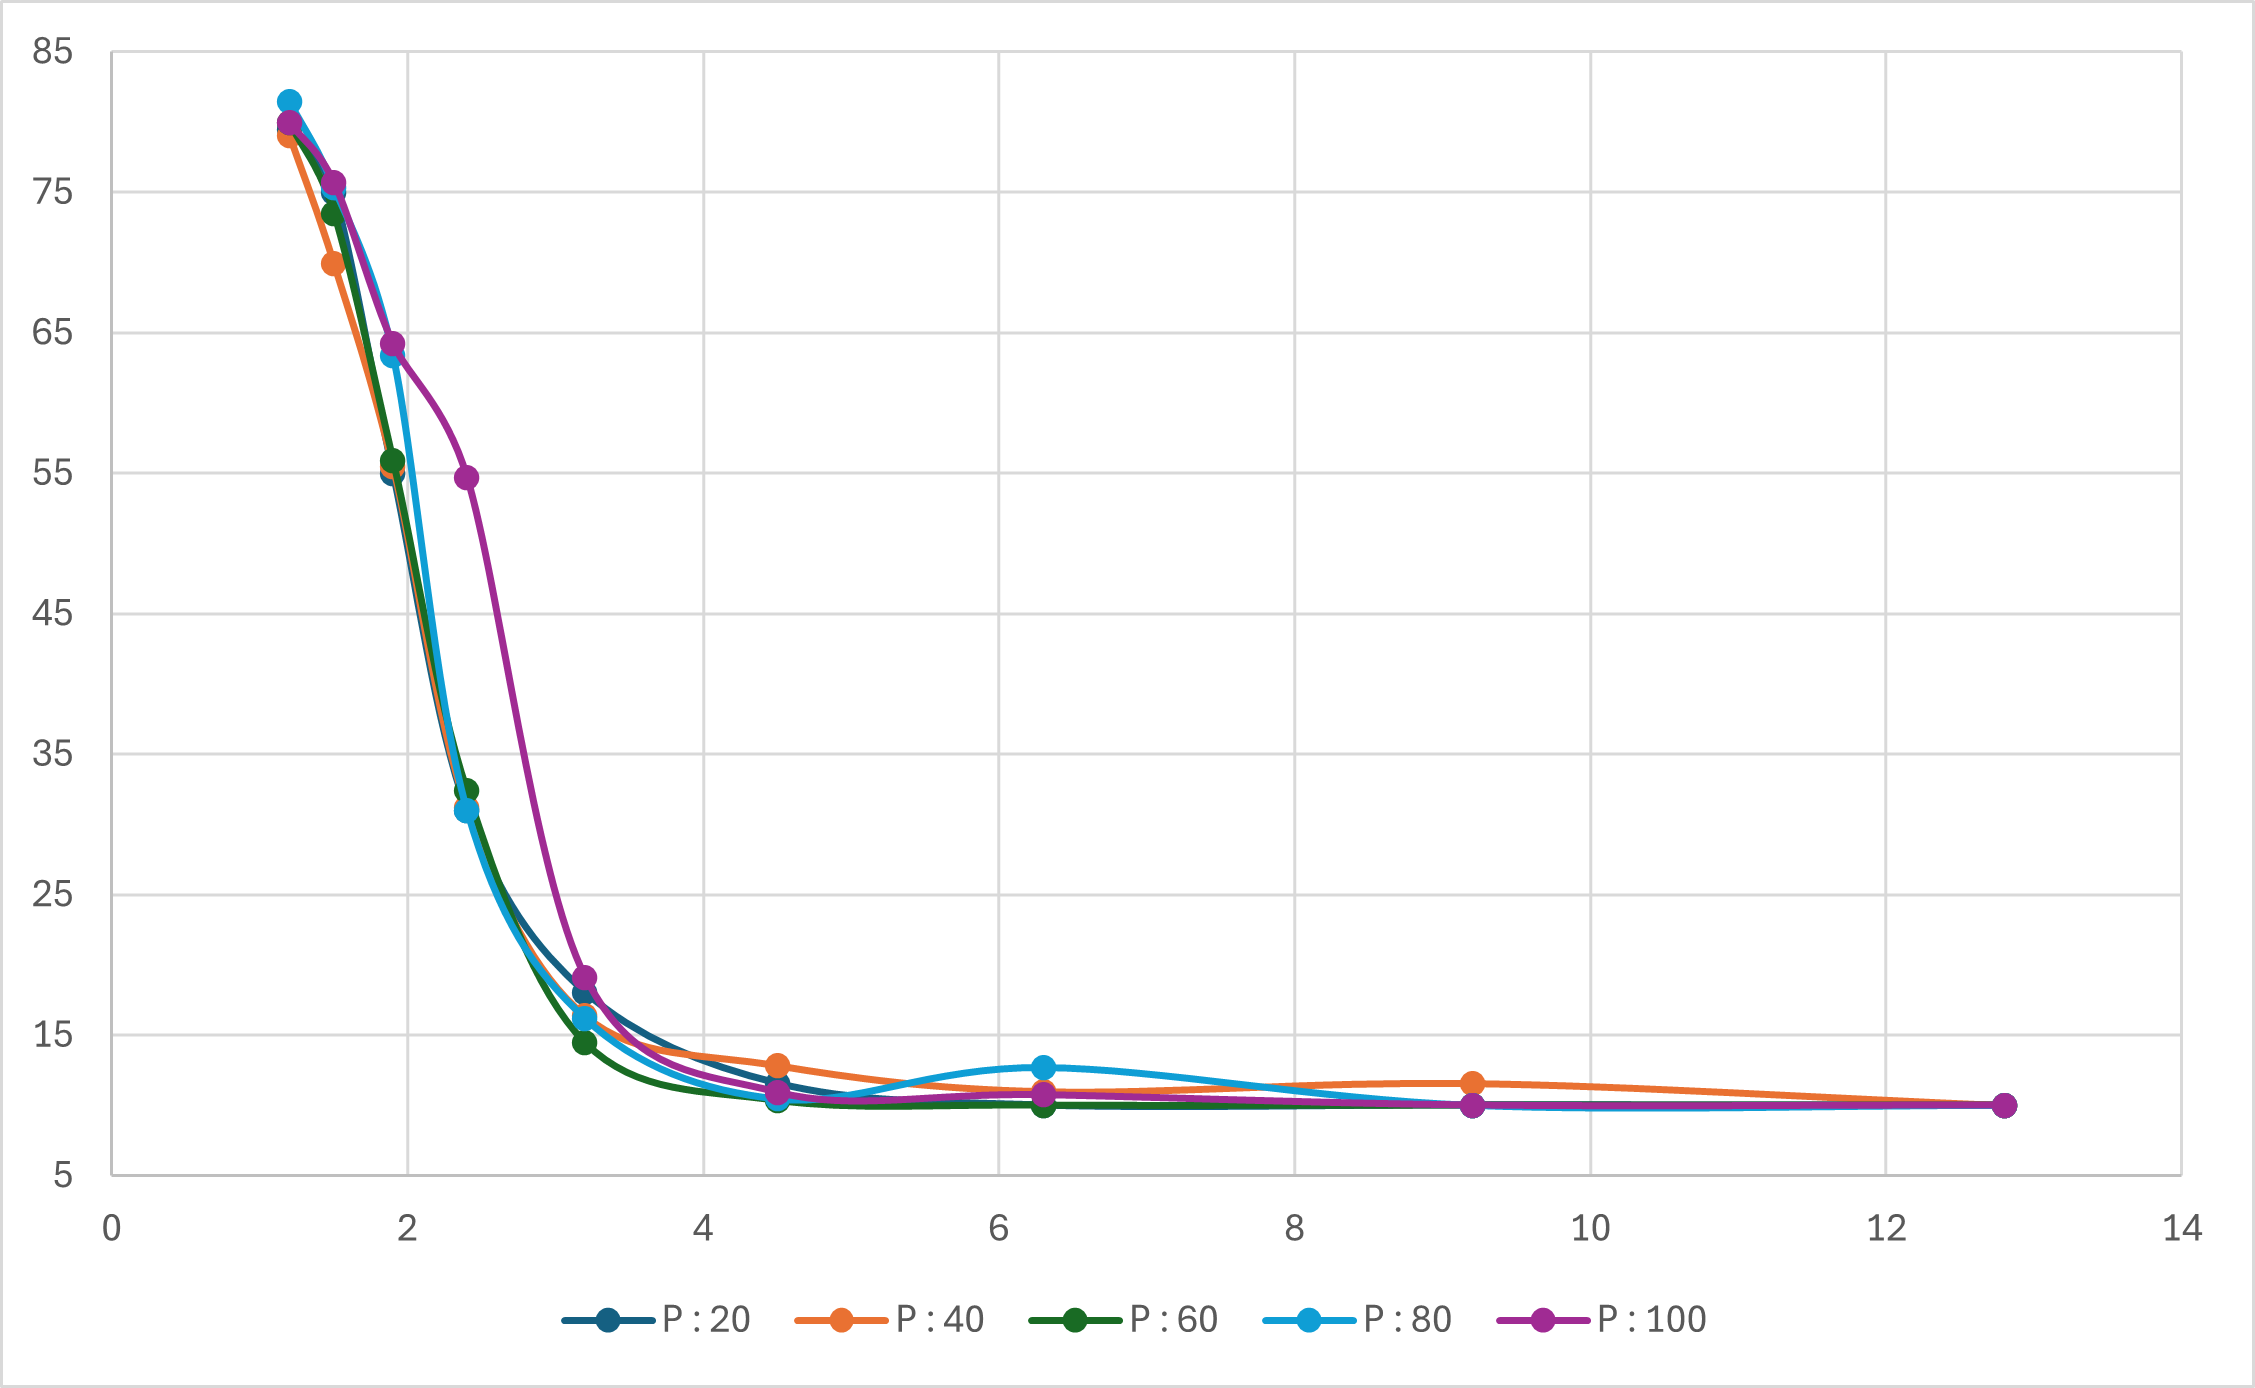
\includegraphics[width=0.7\textwidth]{accuracy_pre_pruning.png} % ajuster la taille
    \caption{Accuracy du modèle entrainé pruné avant fine-tuning pour différentes valeurs de compression} % légende
    \label{fig:mon_image} % label pour référence
\end{figure}
Tout d'abord, nous constatons que la pour tout valeurs de P, la courbe possède une variation et une pente similaire. En particulier, un calcul d'écart quadratique à la moyenne, montre une variation d'accuracy moyenne par niveau de compression de 3.89. L'accuracy est maximal sur à chaque niveau de compression pour des valeurs de P différentes. Aussi, l'accuracy chute à partir d'une compression égale à 2. Plus précisement, la pente est maximale pour le niveau de compression 2,4, à l'exception de P = 100. A partir du niveau de compression 4, l'accuracy pour toute valeur de P est proche de 10 \%, le modèle est aléatoire aussi performante qu'un tirage aléatoire (10 classes).
La valeur maximal d'accuracy, obtenue pour la plus petite compression, avoisine les 80 \% pour P = 80. Comparons à présente, avec les méthodes benchmarks de pruning : 
\begin{figure}[H] % h = "here", pour placer l'image ici
    \centering    % centre l'image
    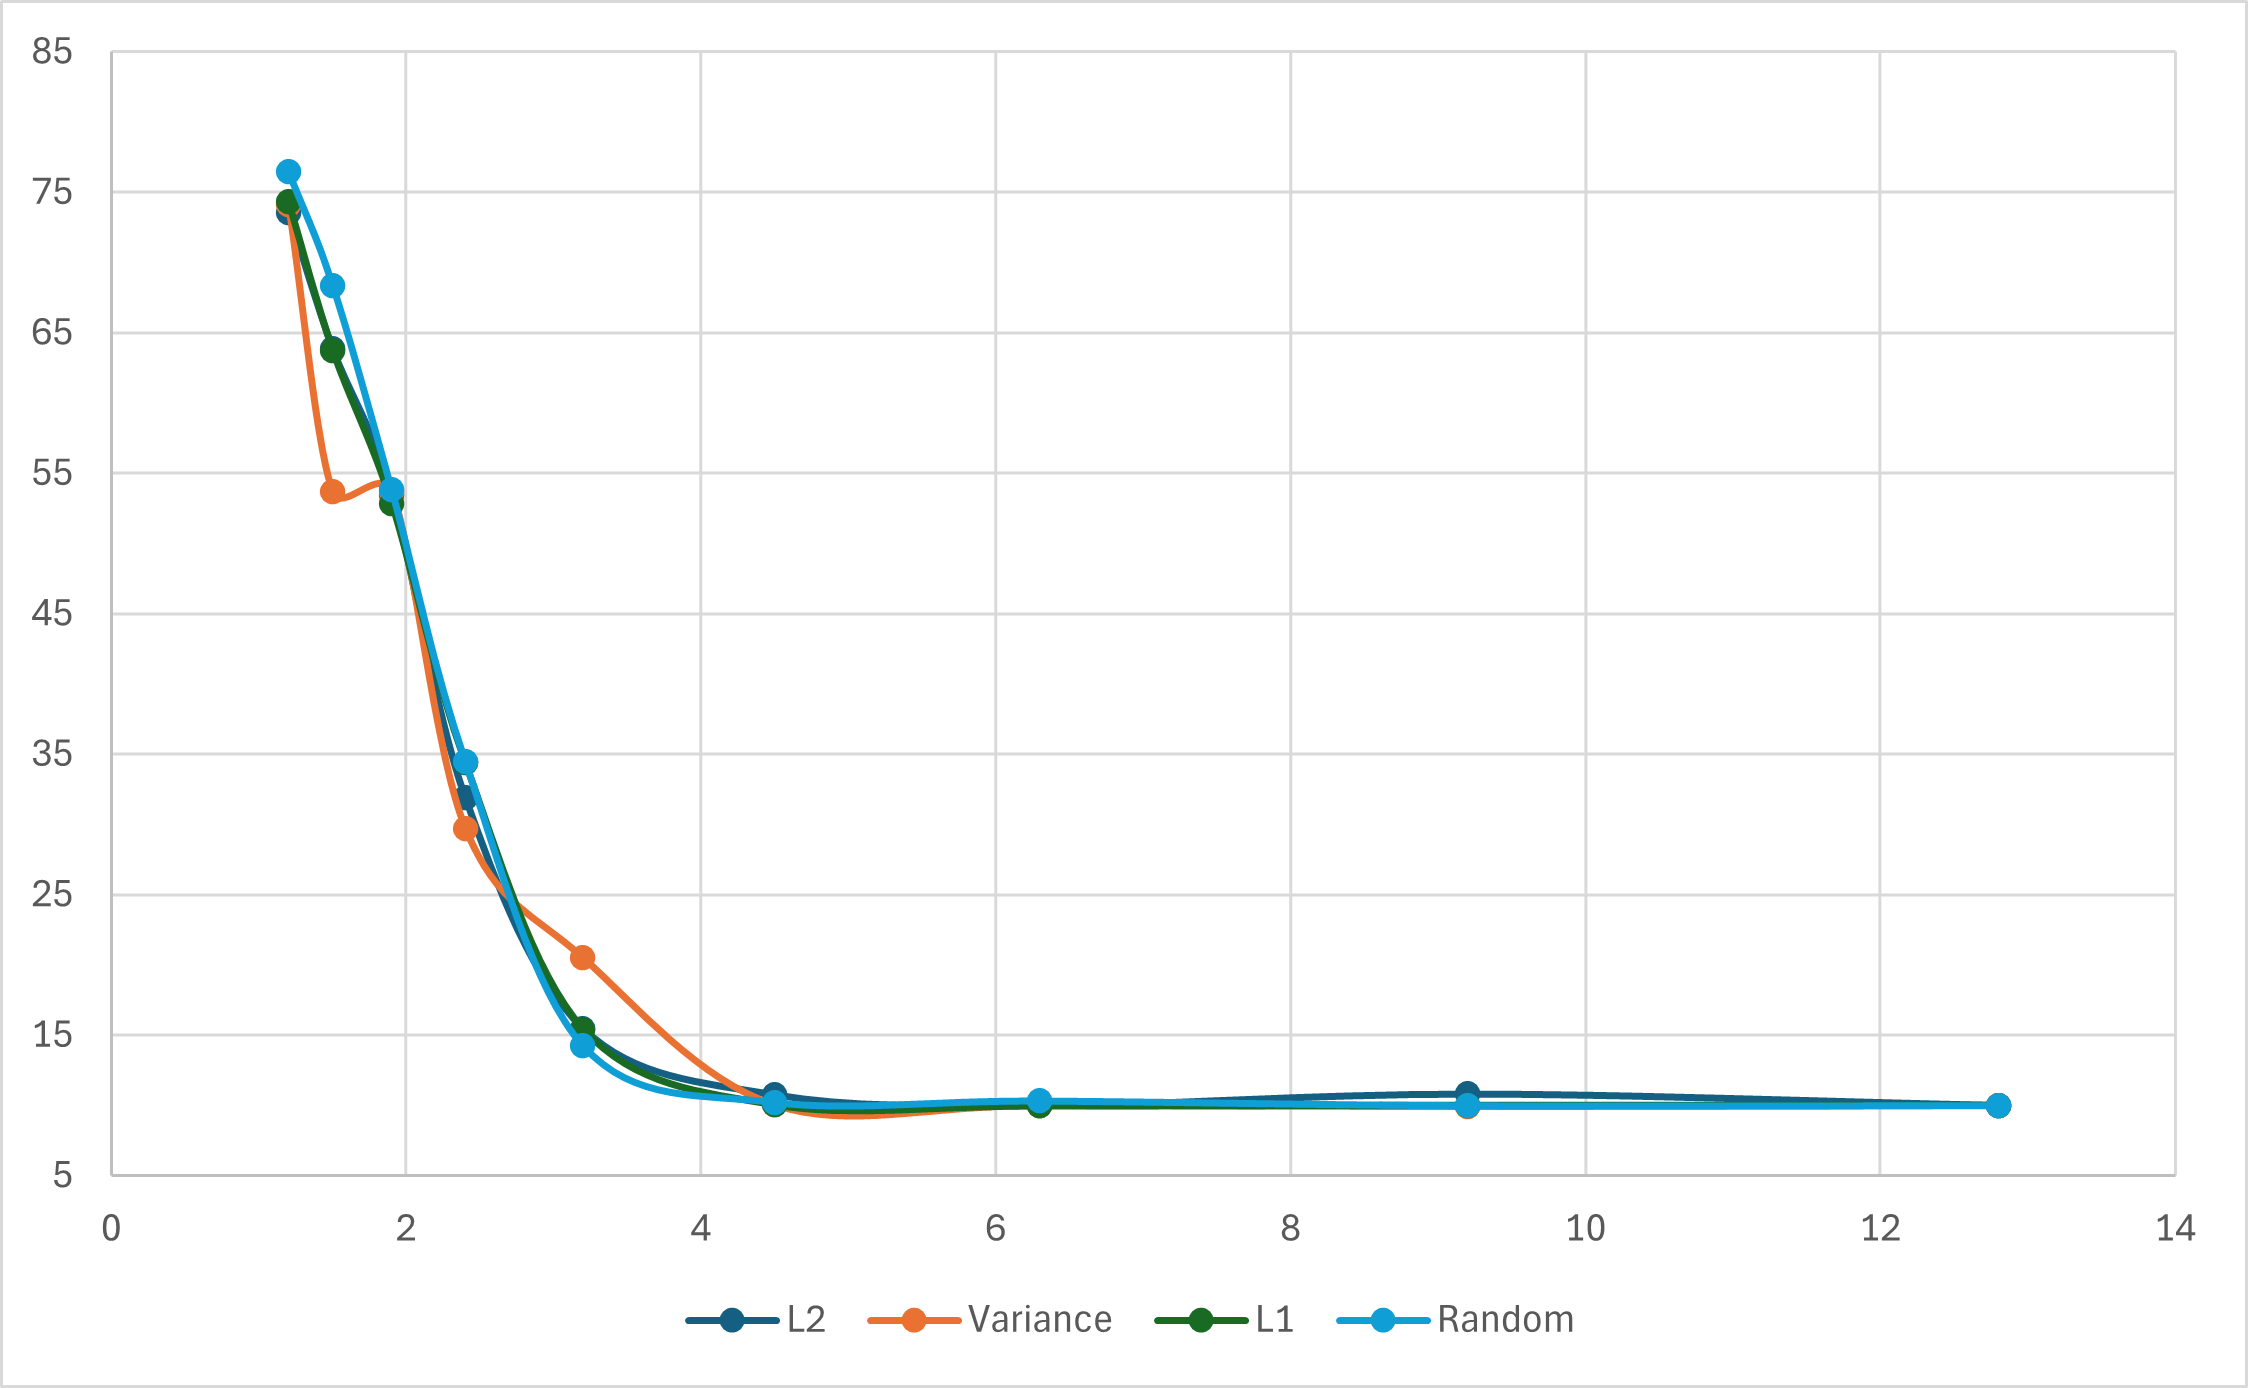
\includegraphics[width=0.7\textwidth]{accuracy_pre_pruning_benchmark.png} % ajuster la taille
    \caption{Accuracy du modèle entrainé pruné par méthodes standards avant fine-tuning pour différentes valeurs de compression} % légende
    \label{fig:mon_image} % label pour référence
\end{figure}
Nous constatons que les méthodes standards de pruning suivent une tendance similaire à notre méthode de pruning. En effet, en moyennant les résultats d'accuracy pour les différentes valeurs de P et pour les différentes méthodes de pruning standards, nous calculons une corrélation de Pearson de 0.9950. Au delà de cette corrélation, il est étonnant de constater que des mesures fondamentalement différentes des poids des filtres fournissent une évaluation similaire de l'accuracy du modèle. En effet, un calcul de l'écart quadratique moyenne pour les 4 méthodes, nous donne un écart moyen 2.09 point d'accuracy par mesure. Filtrer de manière aléatoire est en ce sens aussi performant voire localement plus performante que de mesurer par les normes L1, L2 ou par variance. Ce constat nous permet d'affirmer, dans le cas de notre modèle, que le pruning L1, L2 et par variance ne sont pas des mesures fiables d'importances des filtres du modèle. 
Globalement, les résultats avant fine-tuning des méthodes standards atteigne le plateau des 10 \% d'accuracy plus rapidement que pour notre méthode de pruning et presente une accuracy maximale plus faible à 76,5\% contre 81.42 \% pour notre méthode pour P = 80. 
\begin{figure}[H] % h = "here", pour placer l'image ici
    \centering    % centre l'image
    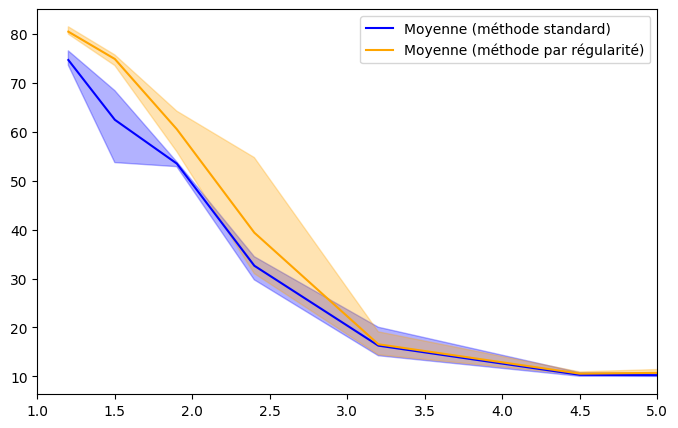
\includegraphics[width=0.7\textwidth]{comparaison_benchmark_model.png} % ajuster la taille
    \caption{Comparaison des modèles de pruning avant fine-tuning pour niveau de compression inférieur à 4} % légende
    \label{fig:mon_image} % label pour référence
\end{figure}
Ci-dessus, le graphique représente l'accuracy moyenne des méthodes standard et des méthodes par régularité pour les différentes valeurs de P. Le canal, représente les valeurs minimales et maximale pour ces deux méthodes. Ainsi, nous constatons que avant fine-tuning, notre méthode d'analyse des filtres par régularité permet 
d'obtenir en moyenne une meilleur accuracy jusqu'au niveau de compression 3 puis similaire puis une accuracy similaire pour les niveaux de compressions supérieures. 
\begin{figure}[H] % h = "here", pour placer l'image ici
    \centering    % centre l'image
    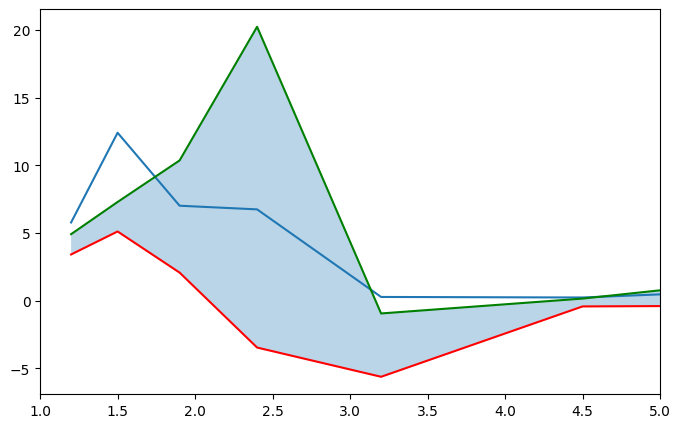
\includegraphics[width=0.7\textwidth]{difference_accuracy_entre_model_pre_tuning.png} % ajuster la taille
    \caption{Difference d'accuracy entre les moyennes des méthodes standards et de régularités} % légende
    \label{fig:mon_image} % label pour référence
\end{figure}
Le graphique ci-dessus représente l'écart d'accuracy entre notre modèle et les modèles standards. La courbe bleu représente l'écart moyen entre l'ensemble des modèles de régularités et des modèles standards. Sur l'ensemble de la plage de compression, notre modèle surpasse en moyenne de 3,7 point d'accuracy les modèles standards, la version la plus précise de notre modèle elle surpasse de 4.84 cette moyenne. 
La courbe verte représente la différence d'accuracy entre le modèle de régularité le plus précis et le modèle standard le plus précis. La courbe rouge représente la différence d'accuracy entre le modèle de régularité le moins précis et le modèle standard le plus précis. Ainsi nous constatons que toutes les versions du modèles de régularités ne surpassent pas en accuracy les modèles standards. 

\begin{figure}[H] % h = "here", pour placer l'image ici
    \centering    % centre l'image
    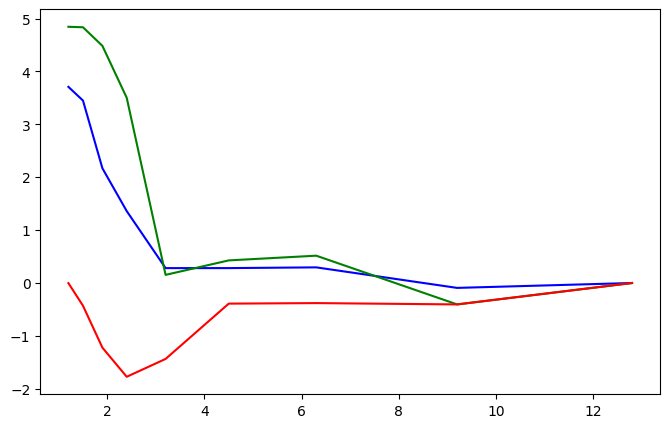
\includegraphics[width=0.7\textwidth]{moyenne_glissante_pre_tuning.png} % ajuster la taille
    \caption{Moyenne glissante de la différence d'accuracy entre les modèles} % légende
    \label{fig:mon_image} % label pour référence
\end{figure}
Le graphique ci-dessus représente la moyenne glissante de différence d'accuracy sur les 12 niveaux de compression. Ainsi, nous constatons que la différence d'accuracy est surtout notable sur les 4 premiers niveaux de compression. 
\paragraph{Accuracy après fine-tuning}
Une fois le modèle pruné, nous le fine-tuned sur 5 epochs permet d'augmenter l'accuracy après la suppression des filtres. Le choix du nombre d'epochs est crucial. En effet, nous avons pu observer lors d'un essai précédent non présenté ici, que fine-tuned sur un nombre plus ou égale à la moitié du nombre d'épochs utilisé pour l'entrainément lisser considérablement les valeurs d'accuracy pour les différentes approches rendant imperceptibles le bénéfice de notre méthode. 
Nous sommes arrivés à la conclusion que, parce qu'il s'agit d'étudier le pruning de notre modèle, ce nombre d'epochs devait rester très inférieur au nombres d'epochs d'entrainement. Ici, nous allons ainsi réaliser le fine-tuning sur 5 epochs. Cette fois-ci nous ne mesurons plus l'accuracy du modèle mais la rétention d'accuracy soit le pourcentage d'accuracy conservé du modèle entrainé (84 \%) Les résultats sont les suivants : 
\begin{figure}[H] % h = "here", pour placer l'image ici
    \centering    % centre l'image
    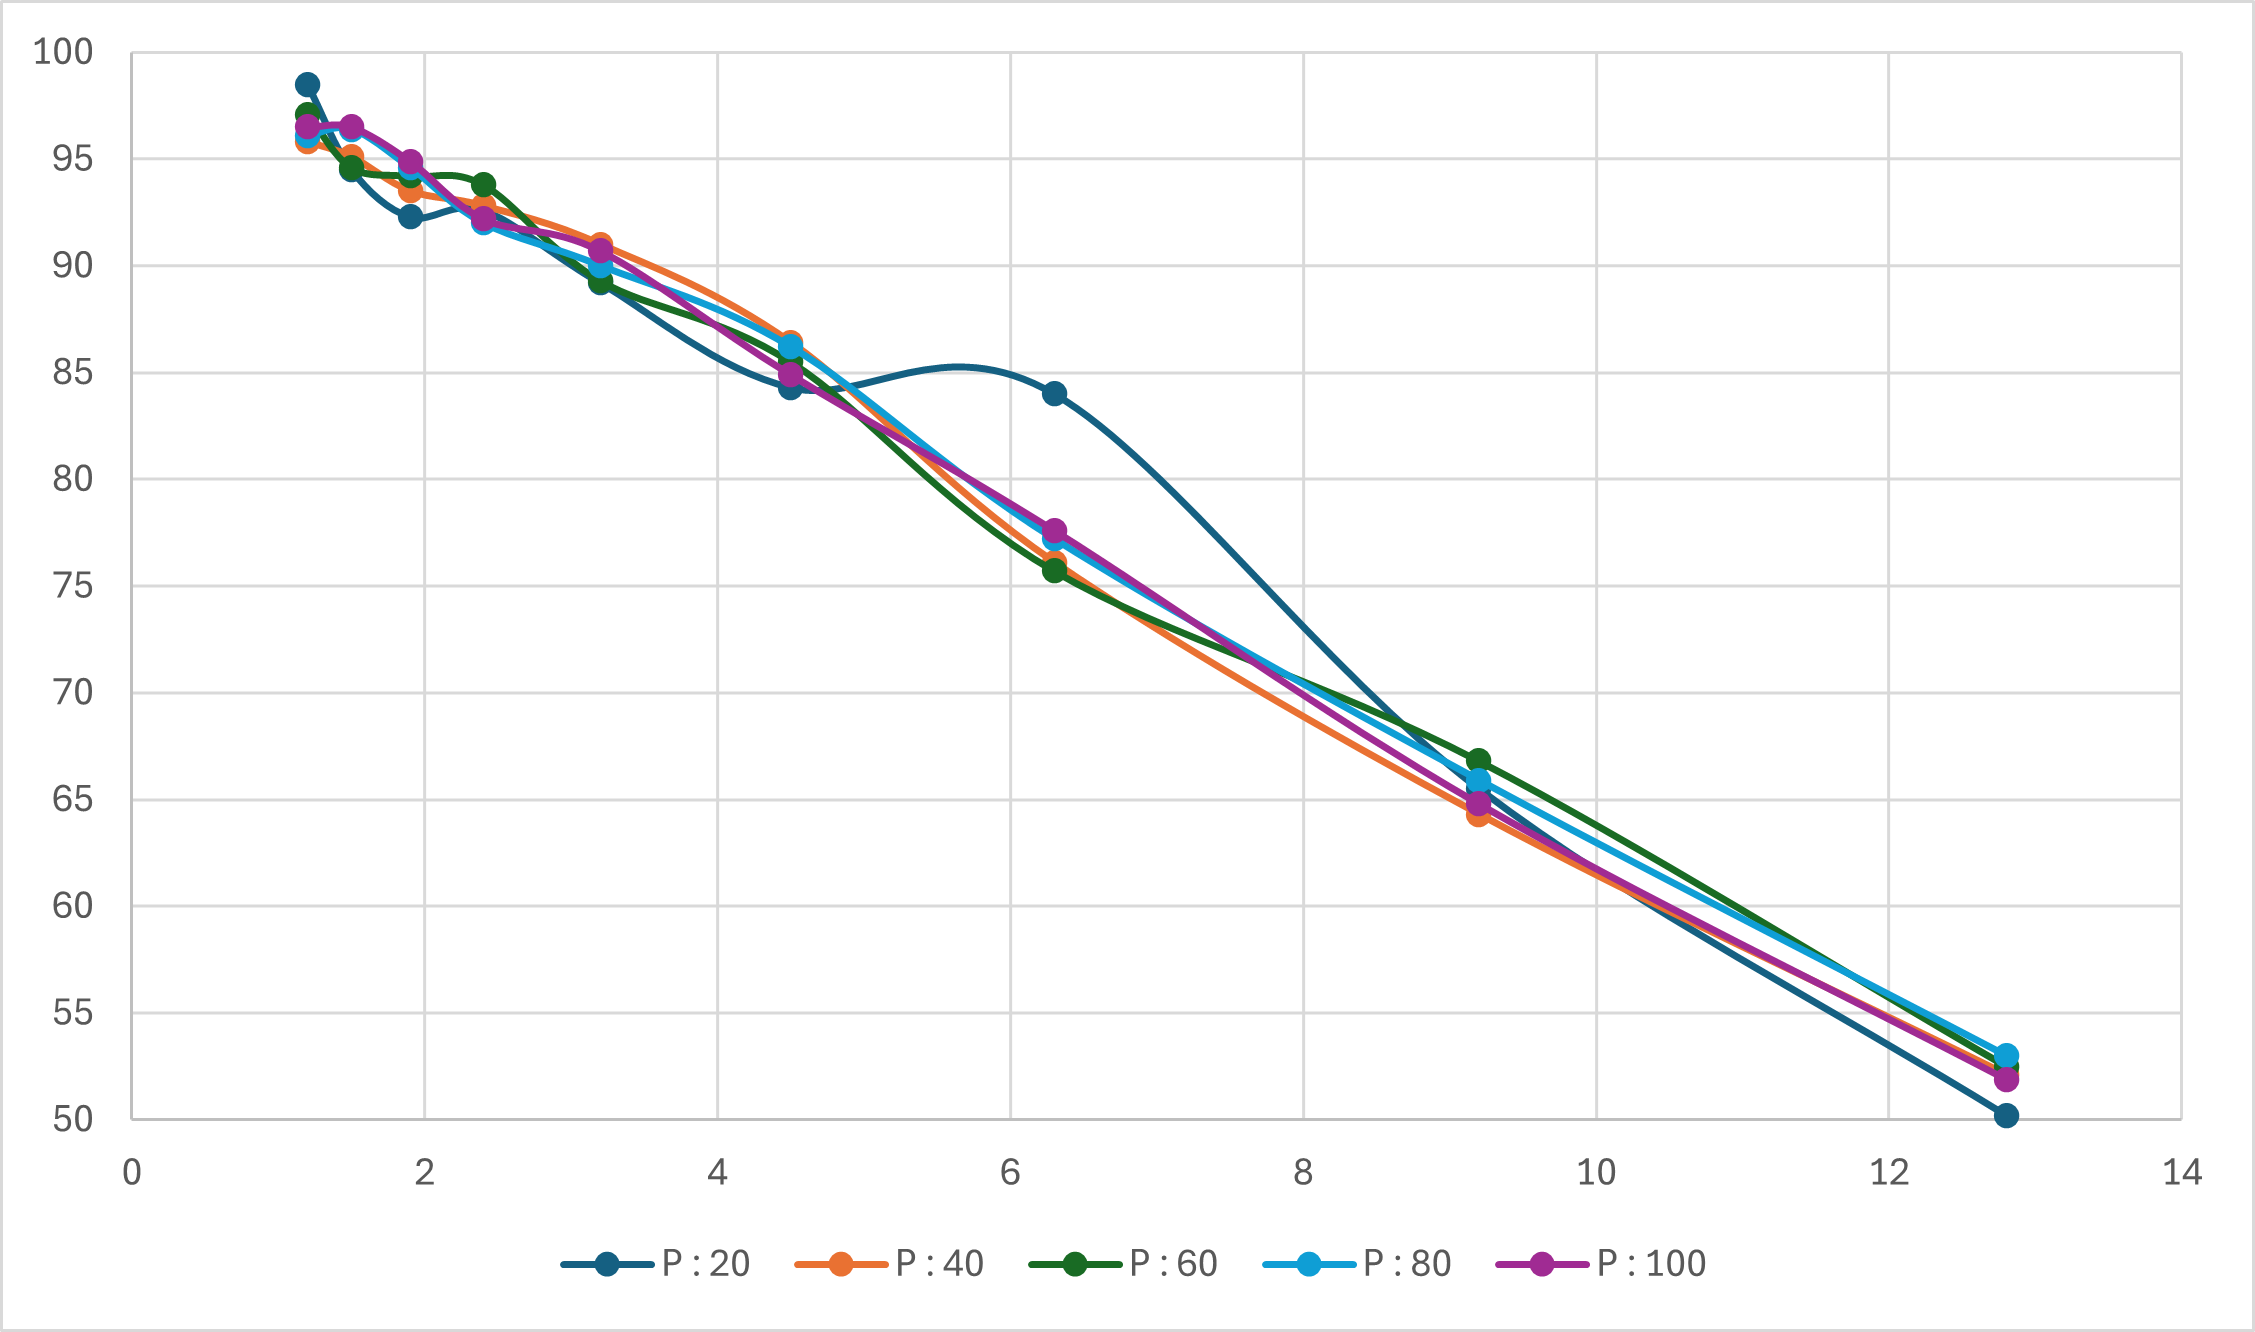
\includegraphics[width=0.7\textwidth]{accuracy_post_pruning.png} % ajuster la taille
    \caption{Accuracy du modèle entrainé pruné après fine-tuning pour différentes valeurs de compression} % légende
    \label{fig:mon_image} % label pour référence
\end{figure}
\begin{figure}[H] % h = "here", pour placer l'image ici
    \centering    % centre l'image
    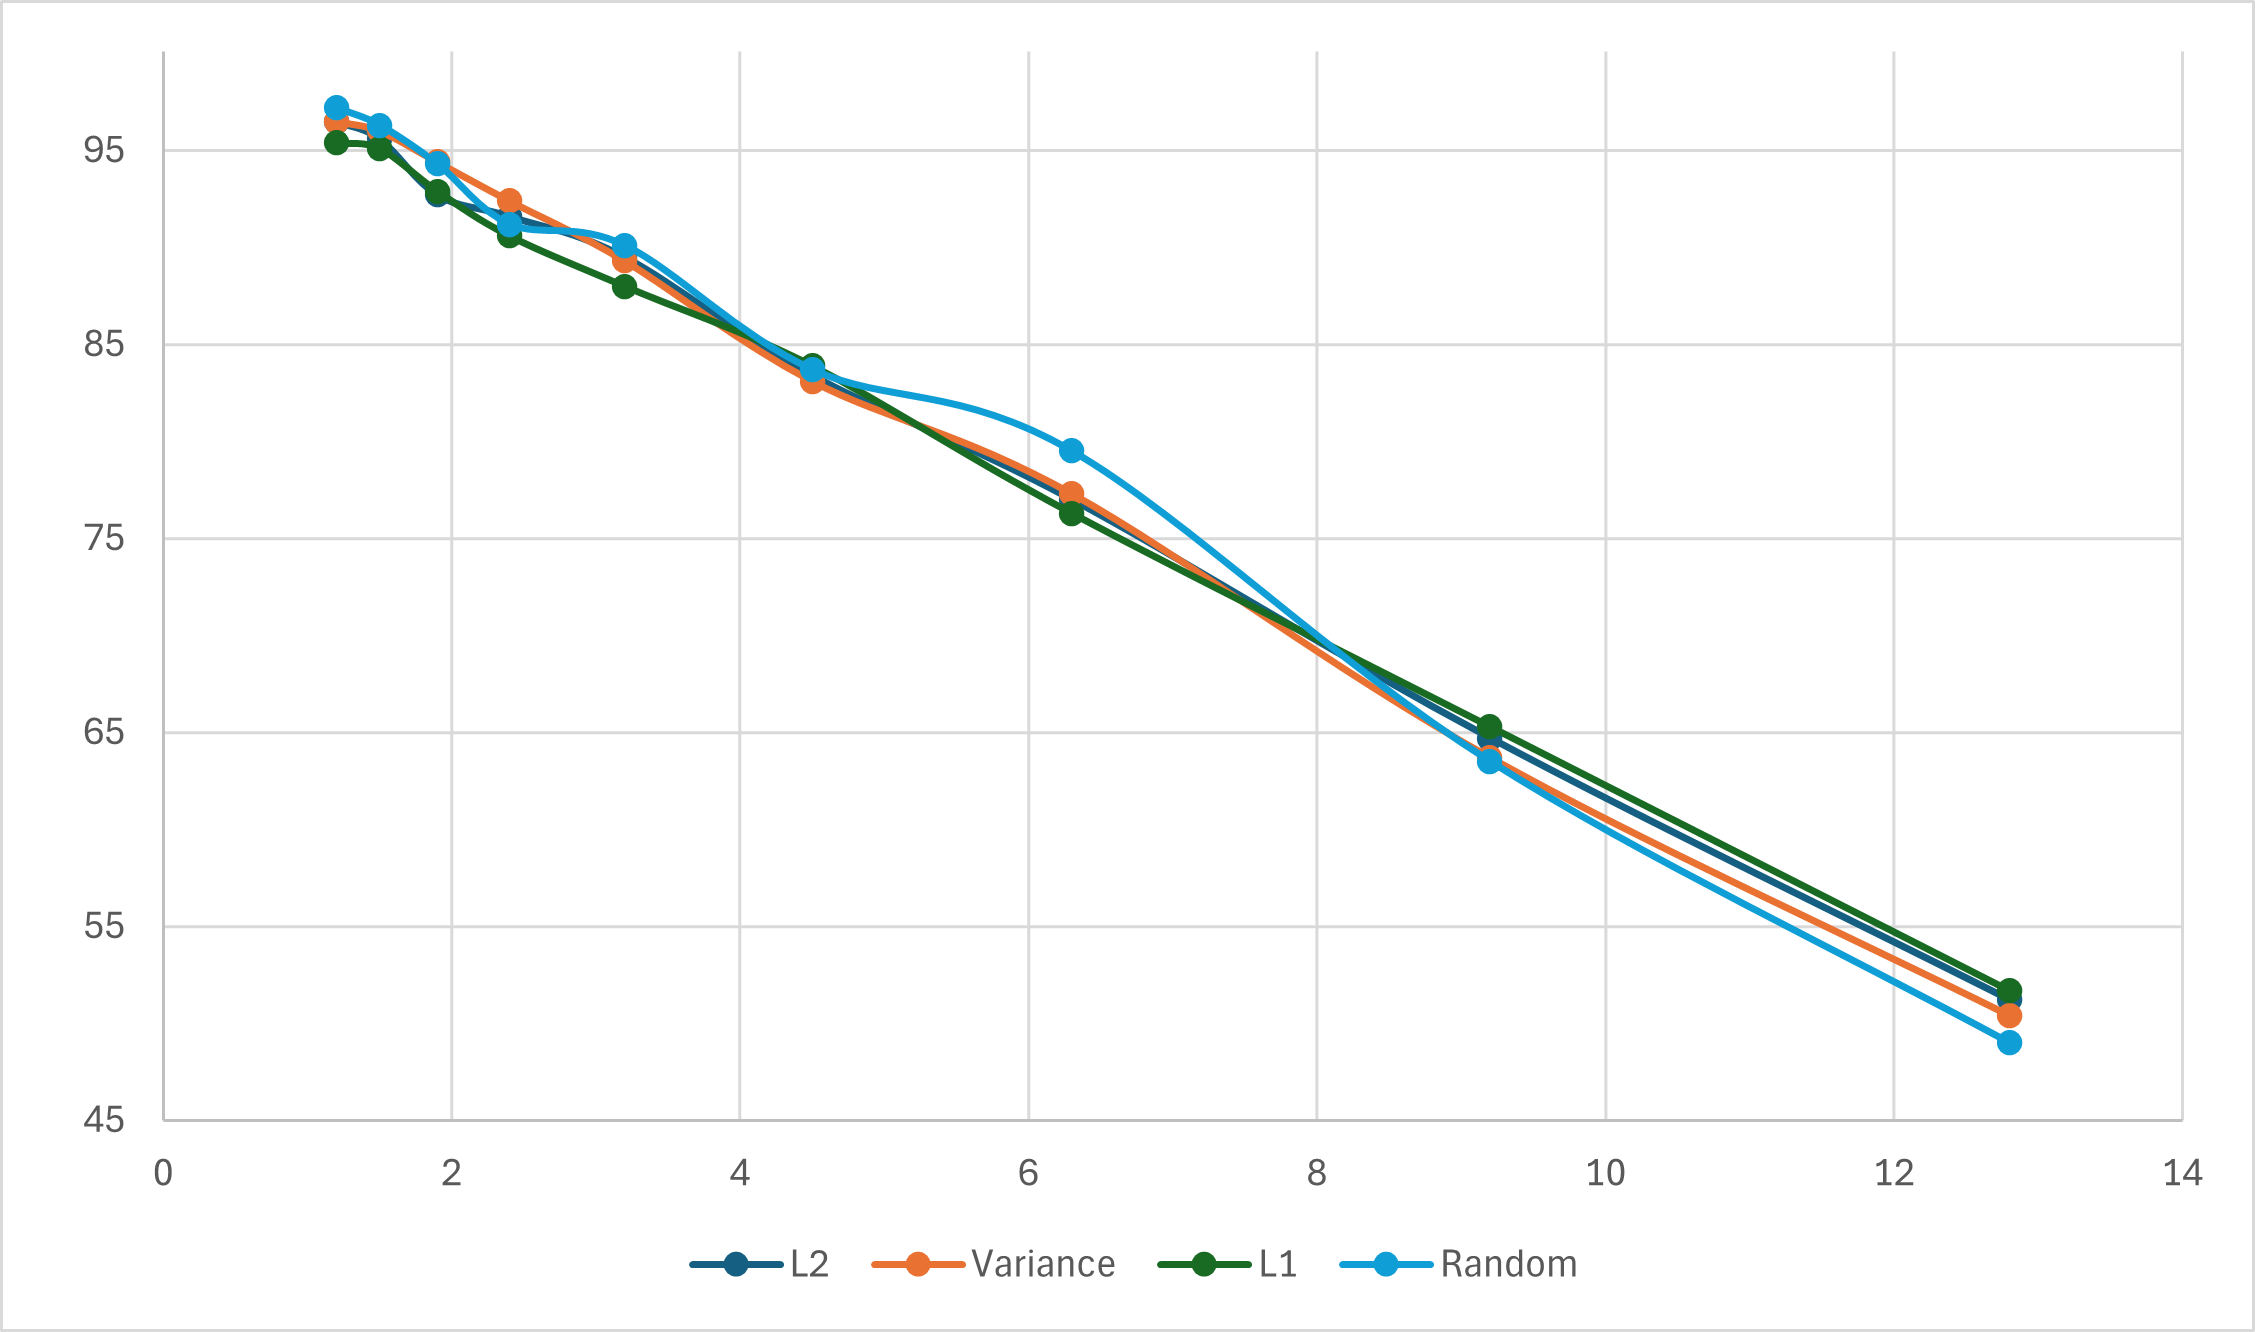
\includegraphics[width=0.7\textwidth]{accuracy_post_pruning_benchmark.png} % ajuster la taille
    \caption{Accuracy du modèle entrainé pruné après fine-tuning pour différentes valeurs de compression des méthodes standards} % légende
    \label{fig:mon_image} % label pour référence
\end{figure}
Nous constatons d'abord que le fine-tuning a "rendu" linéaire les courbes d'accuracy. Une regression linéaire sur la moyenne des résultats pour les méthodes standard et par régularité (pour les différentes valeurs de P) nous donne la pente de ces courbes soit -3.87 pour le pruning par régularité et -3.98 pour les méthodes standards. 
Une comparaison en moyenne des deux approches, permet de confirmer l'effet de lissage du fine-tuning diminuant la différence entre les deux approches 
\begin{figure}[H] % h = "here", pour placer l'image ici
    \centering    % centre l'image
    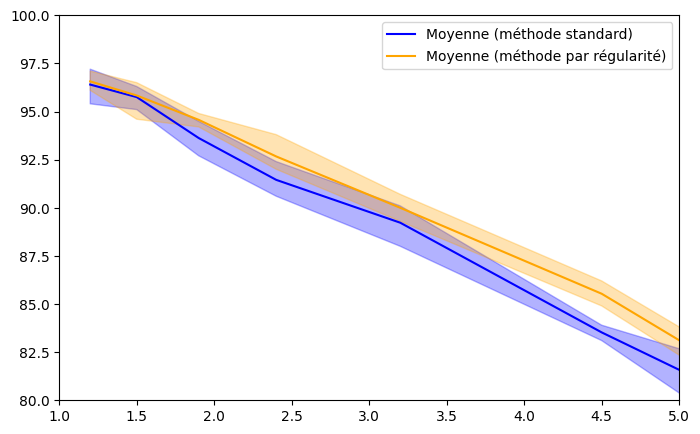
\includegraphics[width=0.7\textwidth]{comparaison_benchmark_model_post.png} % ajuster la taille
    \caption{Comparaison, en moyenne, des modèles de pruning après fine-tuning} % légende
    \label{fig:mon_image} % label pour référence
\end{figure}
\begin{figure}[H] % h = "here", pour placer l'image ici
    \centering    % centre l'image
    \includegraphics[width=0.7\textwidth]{comparaison_benchmark_model_post_non_zoomé.png} % ajuster la taille
    \caption{Comparaison des modèles de pruning après fine-tuning pour niveau d'accuracy inférieur à 4} % légende
    \label{fig:mon_image} % label pour référence
\end{figure}
Ainsi, nous constatons que en moyenne notre approche par régularité égale voire surperforme les approches classiques que nous avons utilisés. 
Les courbes ci-dessus réprésente, en effet, non seulement la moyenne d'accuracy des approches standards et par régularité pour différentes valeurs de compression mais aussi respectivement la méthode et la moins performante au sein de le l'accuracy pour chaque méthode. 
\begin{figure}[H] % h = "here", pour placer l'image ici
    \centering    % centre l'image
    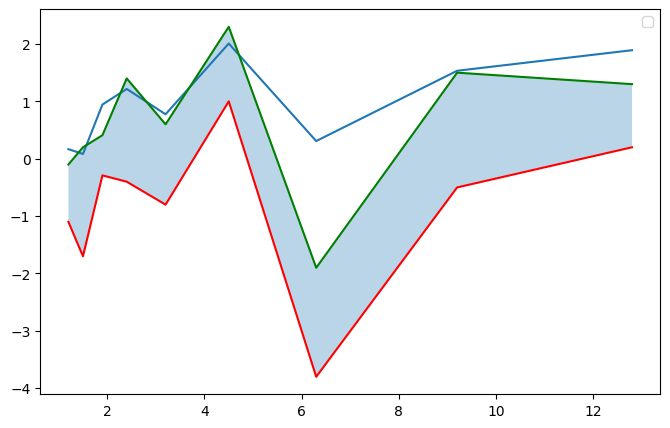
\includegraphics[width=0.7\textwidth]{difference_accuracy_entre_model.png} % ajuster la taille
    \caption{Difference d'accuracy entre les moyennes des méthodes standards et de régularités} % légende
    \label{fig:mon_image} % label pour référence
\end{figure}
Ce graphique, nous permet d'observer l'évolution de la performance de notre modèle en comparaison avec les méthodes standards. 
En particulier, que notre modèle est pour toutes valeurs de compression plus performantes que la moyenne des modèles standards. Plus précisement, la courbe verte représente la différence d'accuracy entre le meilleur modèle de régularité (rappellons que nous fait plusieurs mesure en fonction de la quantité d'information de régularité gardés par filtre) et le meilleur modèle standard. 
Aussi, sauf pour le niveau de compression 6.3 notre meilleur modèle (au sens de l'accuracy) surperforme le meilleur modèles des méthodes standard. Toutefois, la différence de performance reste faible. La courbe rouge représente la différence d'accuracy entre le modèle de régularité le moins précis et le modèle standards le plus précis. Ainsi, nous constatons l'importance d'avoir filtrer l'information par filtre. En effet, si la méthode par régularité a pu surperformer les méthodes standards, elle est aussi en capacité de les sous-performer relativement à la quantité d'information de régularité sélectionné par filtres. 
\subsection{Conclusion et perspectives}
En créant une mesure de régularité basée sur la transformée de Fourier, nous avons pu distinguer signaux et bruit au sein des filtres et proposer un classement de ces derniers en fonction. La méthode de pruning structurel basé sur cette méthode a finalement confirmé l'hypothèse initial. 
En effet, au cours de cette étude, nous avons constater que la régularité des filtres d'un CNN était aussi importante que la magnitude de ces derniers. Les performances, dans le pruning de notre modèle, de la méthode de régularité suggère enfaite, qu'elle le sera même plus. Toutefois, nous avons effectuer notre étude sur une architecture CNN donnée, concluire plus globalement nécessiterait d'effectuer des tests complémentes sur des couches de convolutions différentes. 
En particulier, notre mesure de régularité repose sur un kernel size supérieur à 3. Il pourrait ainsi être envisageable que notre conclusion ne s'applique qu'à ce type de filtre et ne tienne plus pour un kernel size de 3 ou alors pour un agencement différents des couches de convolutions. 
Aussi, le classement des filtres pourrait être améliorer. En effet, une fois la mesure de régularité construire, nous avons appliqué cette dernière à l'ensemble des filtres et sélectionner les filtres les plus réguliers en fonction. Dès lors, nous indidualisons complétement le traitement des filtres. Cependant, en entrainement c'est bien la complémentarité des poids des filtres qui permettent d'optimiser ces derniers, les filtres étant successivement appliqués couche après couches au résultats des convolution faites dans les couches précédentes.
Il s'agirait ainsi de trouver un moyen de conserver la relation des filtres inter couches, afin que la suppression d'un filtre non régulier ne soit pas préjudiciable à un filtre régulier dans une couche suivante. Bien que le fine-tuning permet de compenser cette effet, il demeure que le traiter à la base de notre méthode permettrait peut-être de mieux bénéficier de l'entrainement initial du modèle. 

\end{document}